\documentclass[10pt,twocolumn,letterpaper]{article}

\usepackage{cvpr}
\usepackage{times}
\usepackage{epsfig}
\usepackage{graphicx}
\usepackage{amsmath}
\usepackage{amssymb}
\usepackage{float}
\usepackage{subfigure}
\usepackage{bm}
\usepackage{algorithm}
\usepackage{tabularx}
\usepackage{algpseudocode}
\usepackage{subfloat}
\usepackage{verbatim}


\usepackage[pagebackref=true,breaklinks=true,letterpaper=true,colorlinks,bookmarks=false]{hyperref}
\usepackage[american]{babel}
\usepackage{microtype}

\hypersetup{
    colorlinks=true,
    linkcolor=blue,
    filecolor=red,
    urlcolor=red,
    citecolor=green,
}

\makeatletter
\usepackage{xspace}
\DeclareRobustCommand\onedot{\futurelet\@let@token\@onedot}
\def\@onedot{\ifx\@let@token.\else.\null\fi\xspace}
\def\eg{\emph{e.g}\onedot}
\def\ie{\emph{i.e}\onedot}
\def\etal{\emph{et al}\onedot}
\makeatother

\def\cvprPaperID{6791}

\def\httilde{\mbox{\tt\raisebox{-.5ex}{\symbol{126}}}}

\renewcommand{\algorithmicrequire}{\textbf{Input:}}
\renewcommand{\algorithmicensure}{\textbf{Output:}}

\begin{document}

\bibliographystyle{plain}


\title{Learning to Cartoonize Using White-box Cartoon Representations\\Supplementary Material}
%\maketitle

\twocolumn[{
%\renewcommand\twocolumn
\maketitle
%\begin{figure*}
\begin{center}
    \centering
    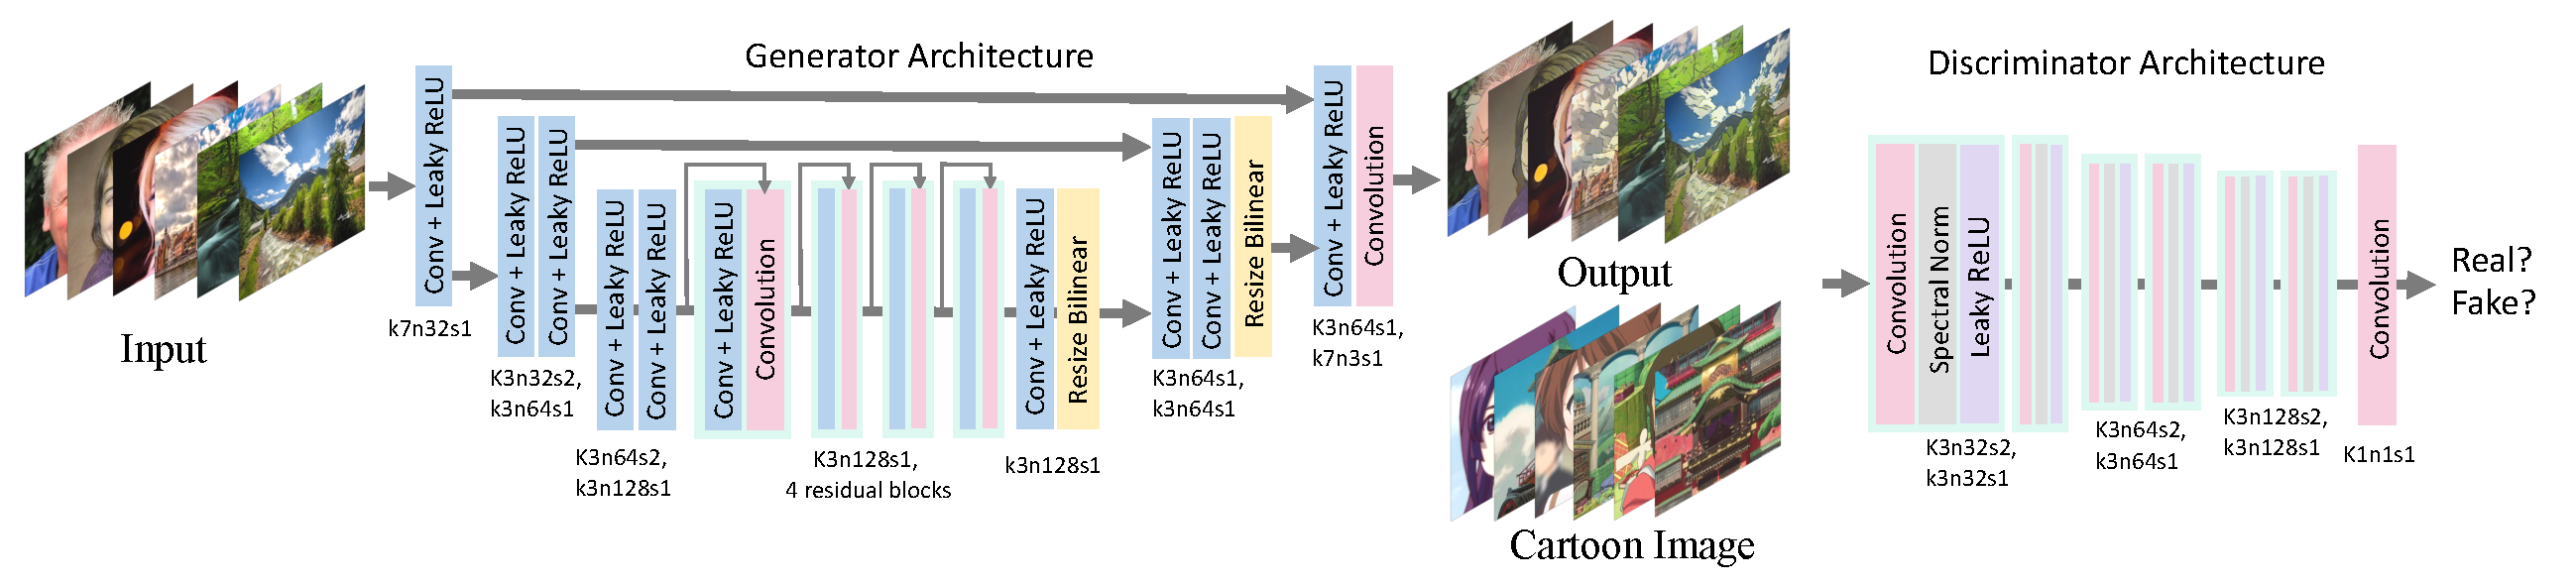
\includegraphics[width=\textwidth]{figures/network_architecture.pdf}
    \captionof{Figure 0.}{ The architecture of generator network and discriminator network.}
    \label{fig:network_architecture}
     \centering
\end{center}
%\end{figure*}
}]


In this supplementary material, we show more experimental results, including the architecture of generator network and discriminator network, results of our method in different use cases, comparison between our results and cartoons in the same scenes, and examples used in the user study. The inference code with pre-trained model and some test images are also submitted for reproducibility.

\vspace{-0.3em}
\section{Network Architecture}
\vspace{-0.3em}
We show the architecture of generator network and discriminator network in Figure \ref{fig:network_architecture}0. The generator network is a fully-convolutional U-Net-like \cite{ronneberger2015u} network. We use convolution layers with stride2 for down-sample and bilinear interpolation layers for upsample to avoid checkerboard artifacts. The network consists of only three kind of layers: convolution,  Leaky ReLU (LReLU) \cite{maas2013rectifier} and bilinear-resize layers. This enables it to be easily embedded in edge devices such as mobile phones. PatchGAN \cite{isola2017image} is adapted in the discriminator network, where the last layer is a convolution layer. Each pixel in the output feature map correspond to a patch in the input image, with the size equals to the perceptive field, and is used to judge whether the patch belongs to cartoon images or generated images. Spectral normalization \cite{miyato2018spectral} is placed after every convolution layer (except the last one) to enforce Lipschitz constrain on the network and stabilize training.

\vspace{-0.3em}
\section{Results in Different Use Cases}
\vspace{-0.3em}
\newpage
In Section 4.1 of the main paper, we apply our method on different scenes and show the cartoonized results. Due to the limitation of space, Only 12 pairs of examples with small resolution are shown. Here we collect images from more use cases with higher resolution, and show the results generated by our method. The content of images includes male celebrities (shown in Figure \ref{fig:person1}), female celebrities (shown in Figure \ref{fig:person2}), food (shown in Figure \ref{fig:food}), sceneries (shown in Figure \ref{fig:scenery1} and Figure \ref{fig:scenery2}), indoors (shown in Figure \ref{fig:home}), city views (shown in Figure \ref{fig:city1} and Figure \ref{fig:city2}), and other objects (shown in Figure \ref{fig:object}). Overall, the above-shown results demonstrate that our method can generate high-quality cartoonized images, and can be applied on diverse use cases and real-world scenes.

\vspace{-0.3em}
\section{Comparison with Cartoon Images}
\vspace{-0.3em}
To further illustrate the cartoonization quality of our method, we present the comparison between the results of our method and cartoon images in the same scene. We collect several cartoon images from Shinkai Makoto's films and their counterpart real-world photos taken in the same scenes. Our method is then applied on the collected real-world photos, and results of our method and cartoon images are shown in Figure \ref{fig:compare1} and Figure \ref{fig:compare2}.

\begin{figure}[t]
%\vspace{-0.5em}
\centering
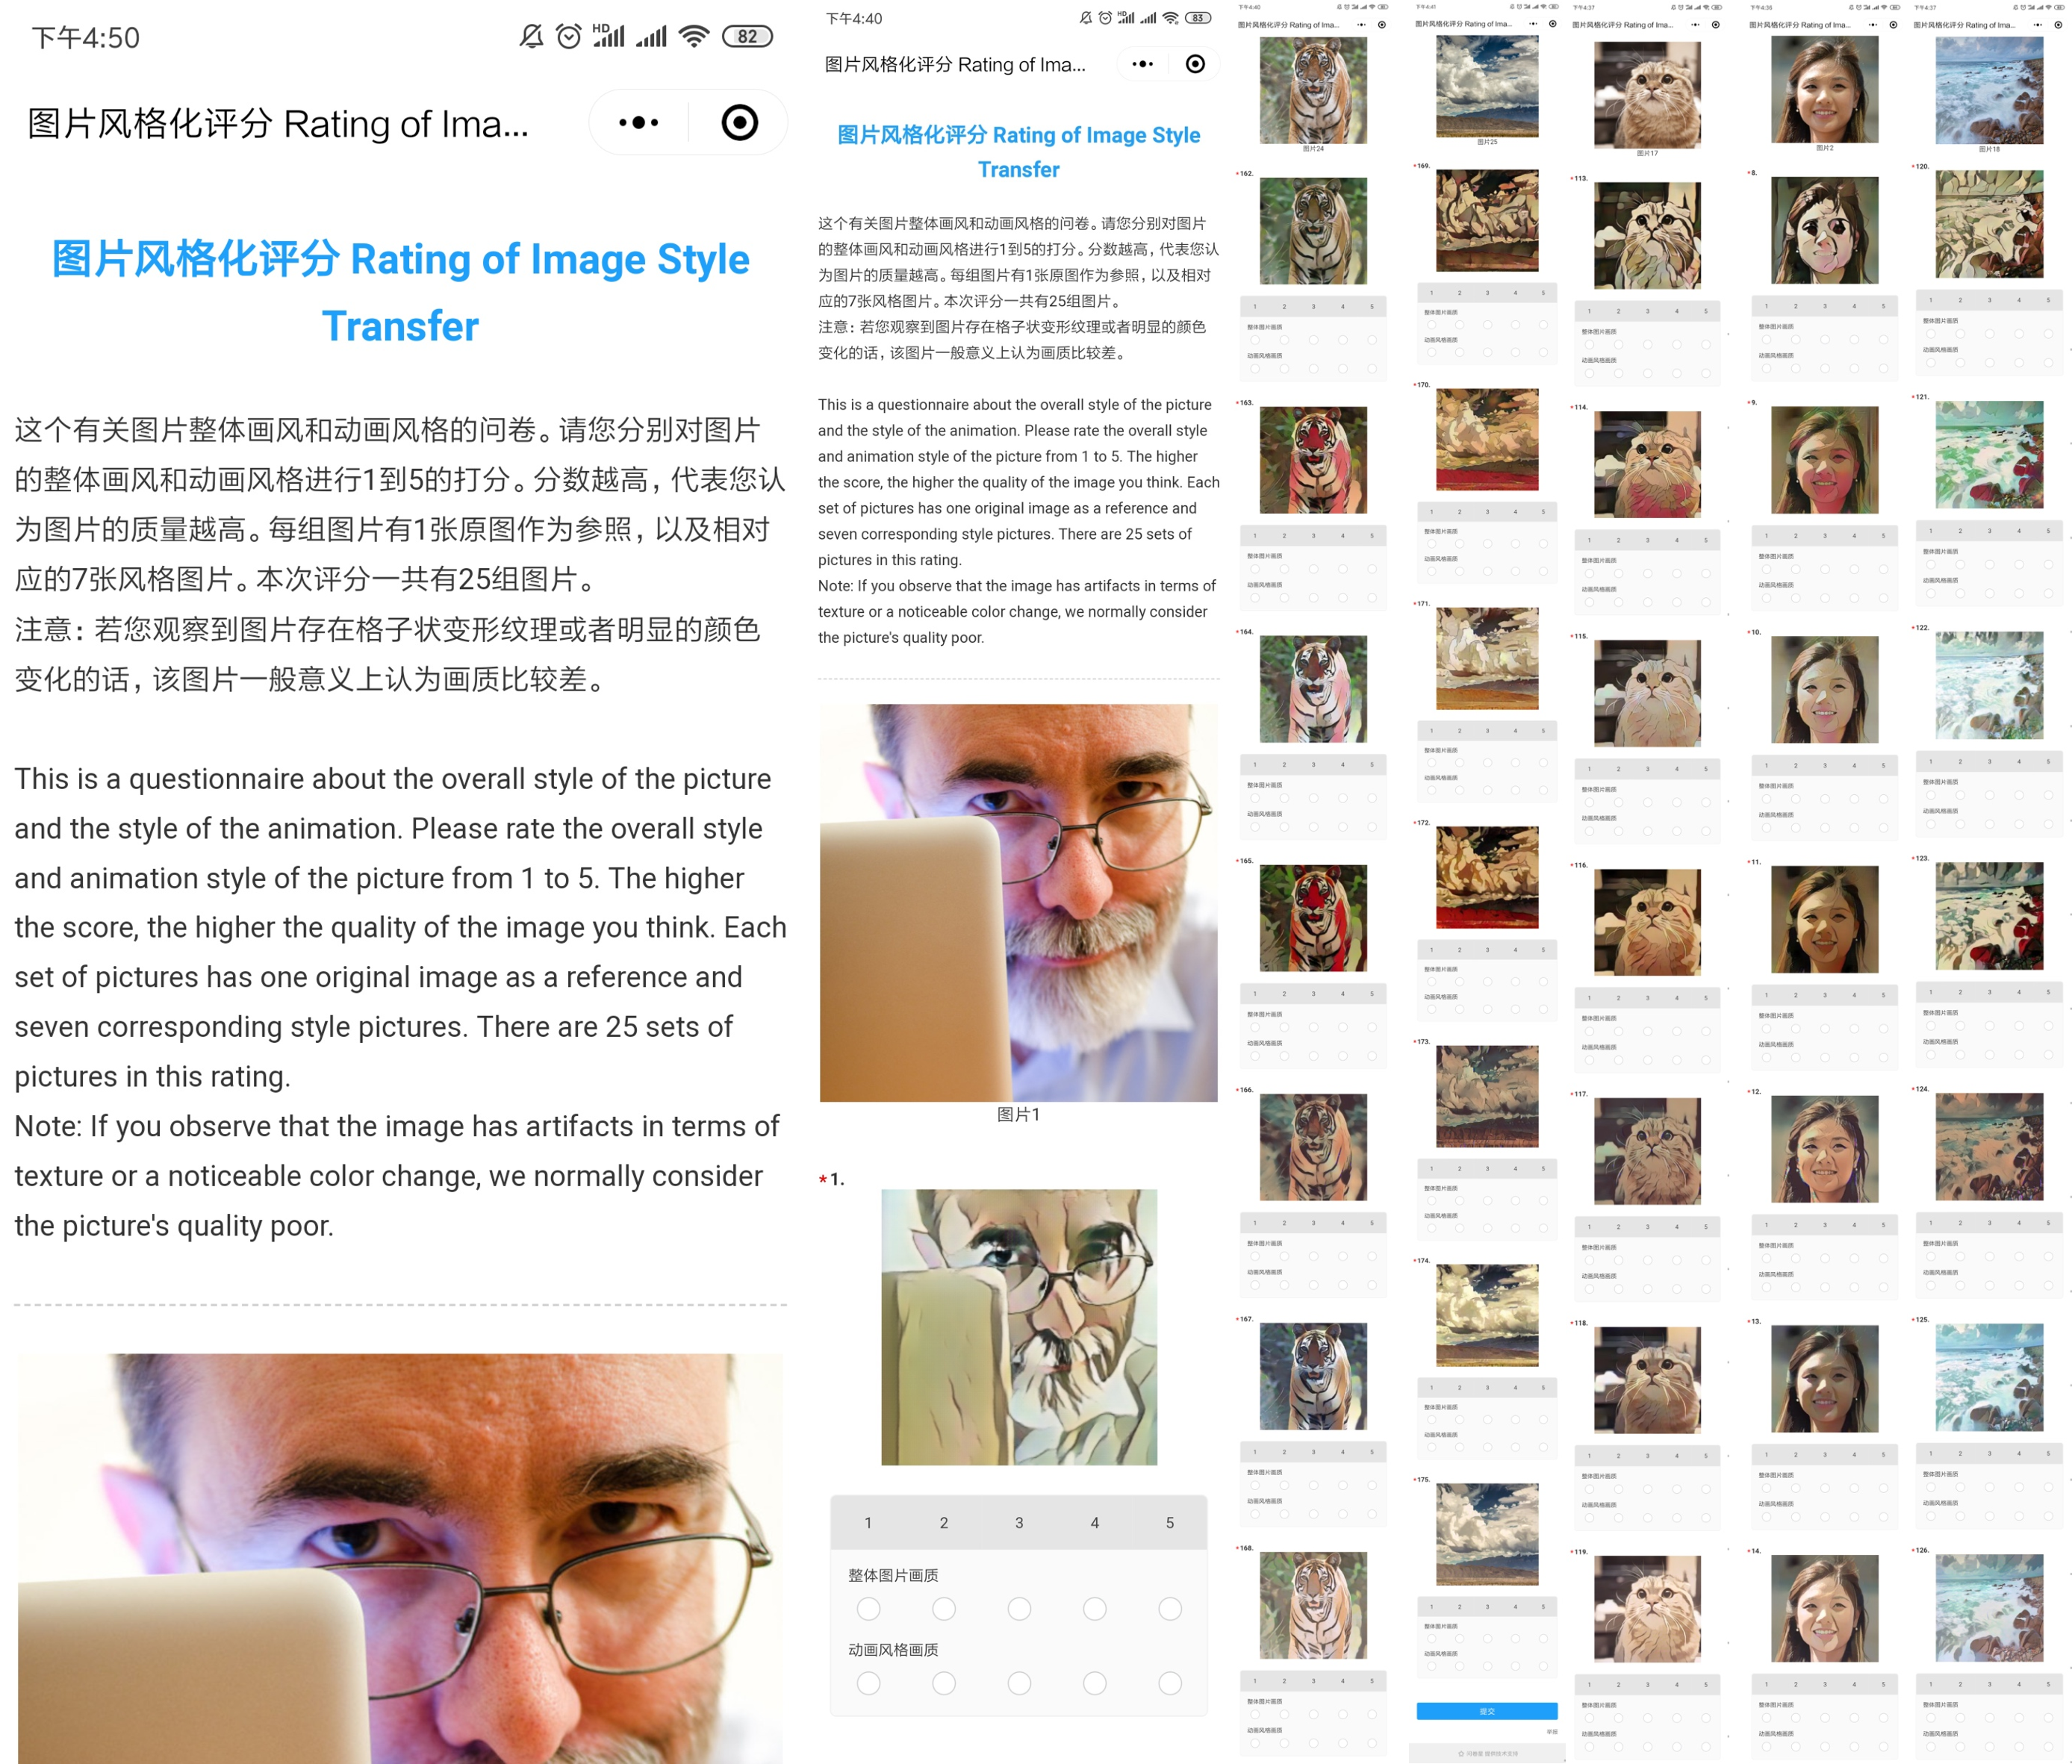
\includegraphics[width=\linewidth]{figures/userstudy_interface.pdf}
\caption{Smartphone application interface of our user study.}
\label{fig:userstudy_interface}
%\vspace{-0.5em}
\end{figure}

\vspace{-0.3em}
\section{Images Shown in the User Study}
\vspace{-0.3em}
We distribute our user study through a smartphone application. The screenshot of the application interface is shown in Figure \ref{fig:userstudy_interface}, and the results of the user study are shown in Figure \ref{fig:userstudy1},  Figure \ref{fig:userstudy2} and  Figure \ref{fig:userstudy3}.

In the user study, we collect 30 images and process them with Fast Neural Style \cite{johnson2016perceptual}, CycleGAN \cite{CycleGAN2017}, CartoonGAN \cite{chen2018cartoongan} and our methods. 10 candidate are asked to score each image from 1 to 5, and the results of user study are shown in the Section 4.4 in the main paper. Here, we show all 30 groups of images processed by different methods, including 8 groups of images with scores. Note that CartoonGAN has 4 styles, and we show them all in the user study, and calculate the average score of the four styles as the final score for CartoonGAN.

\newpage
{\small \bibliographystyle{ieee_fullname} \bibliography{egbib}}

\begin{figure*}[b]
\vspace{-0.5em}
\centering
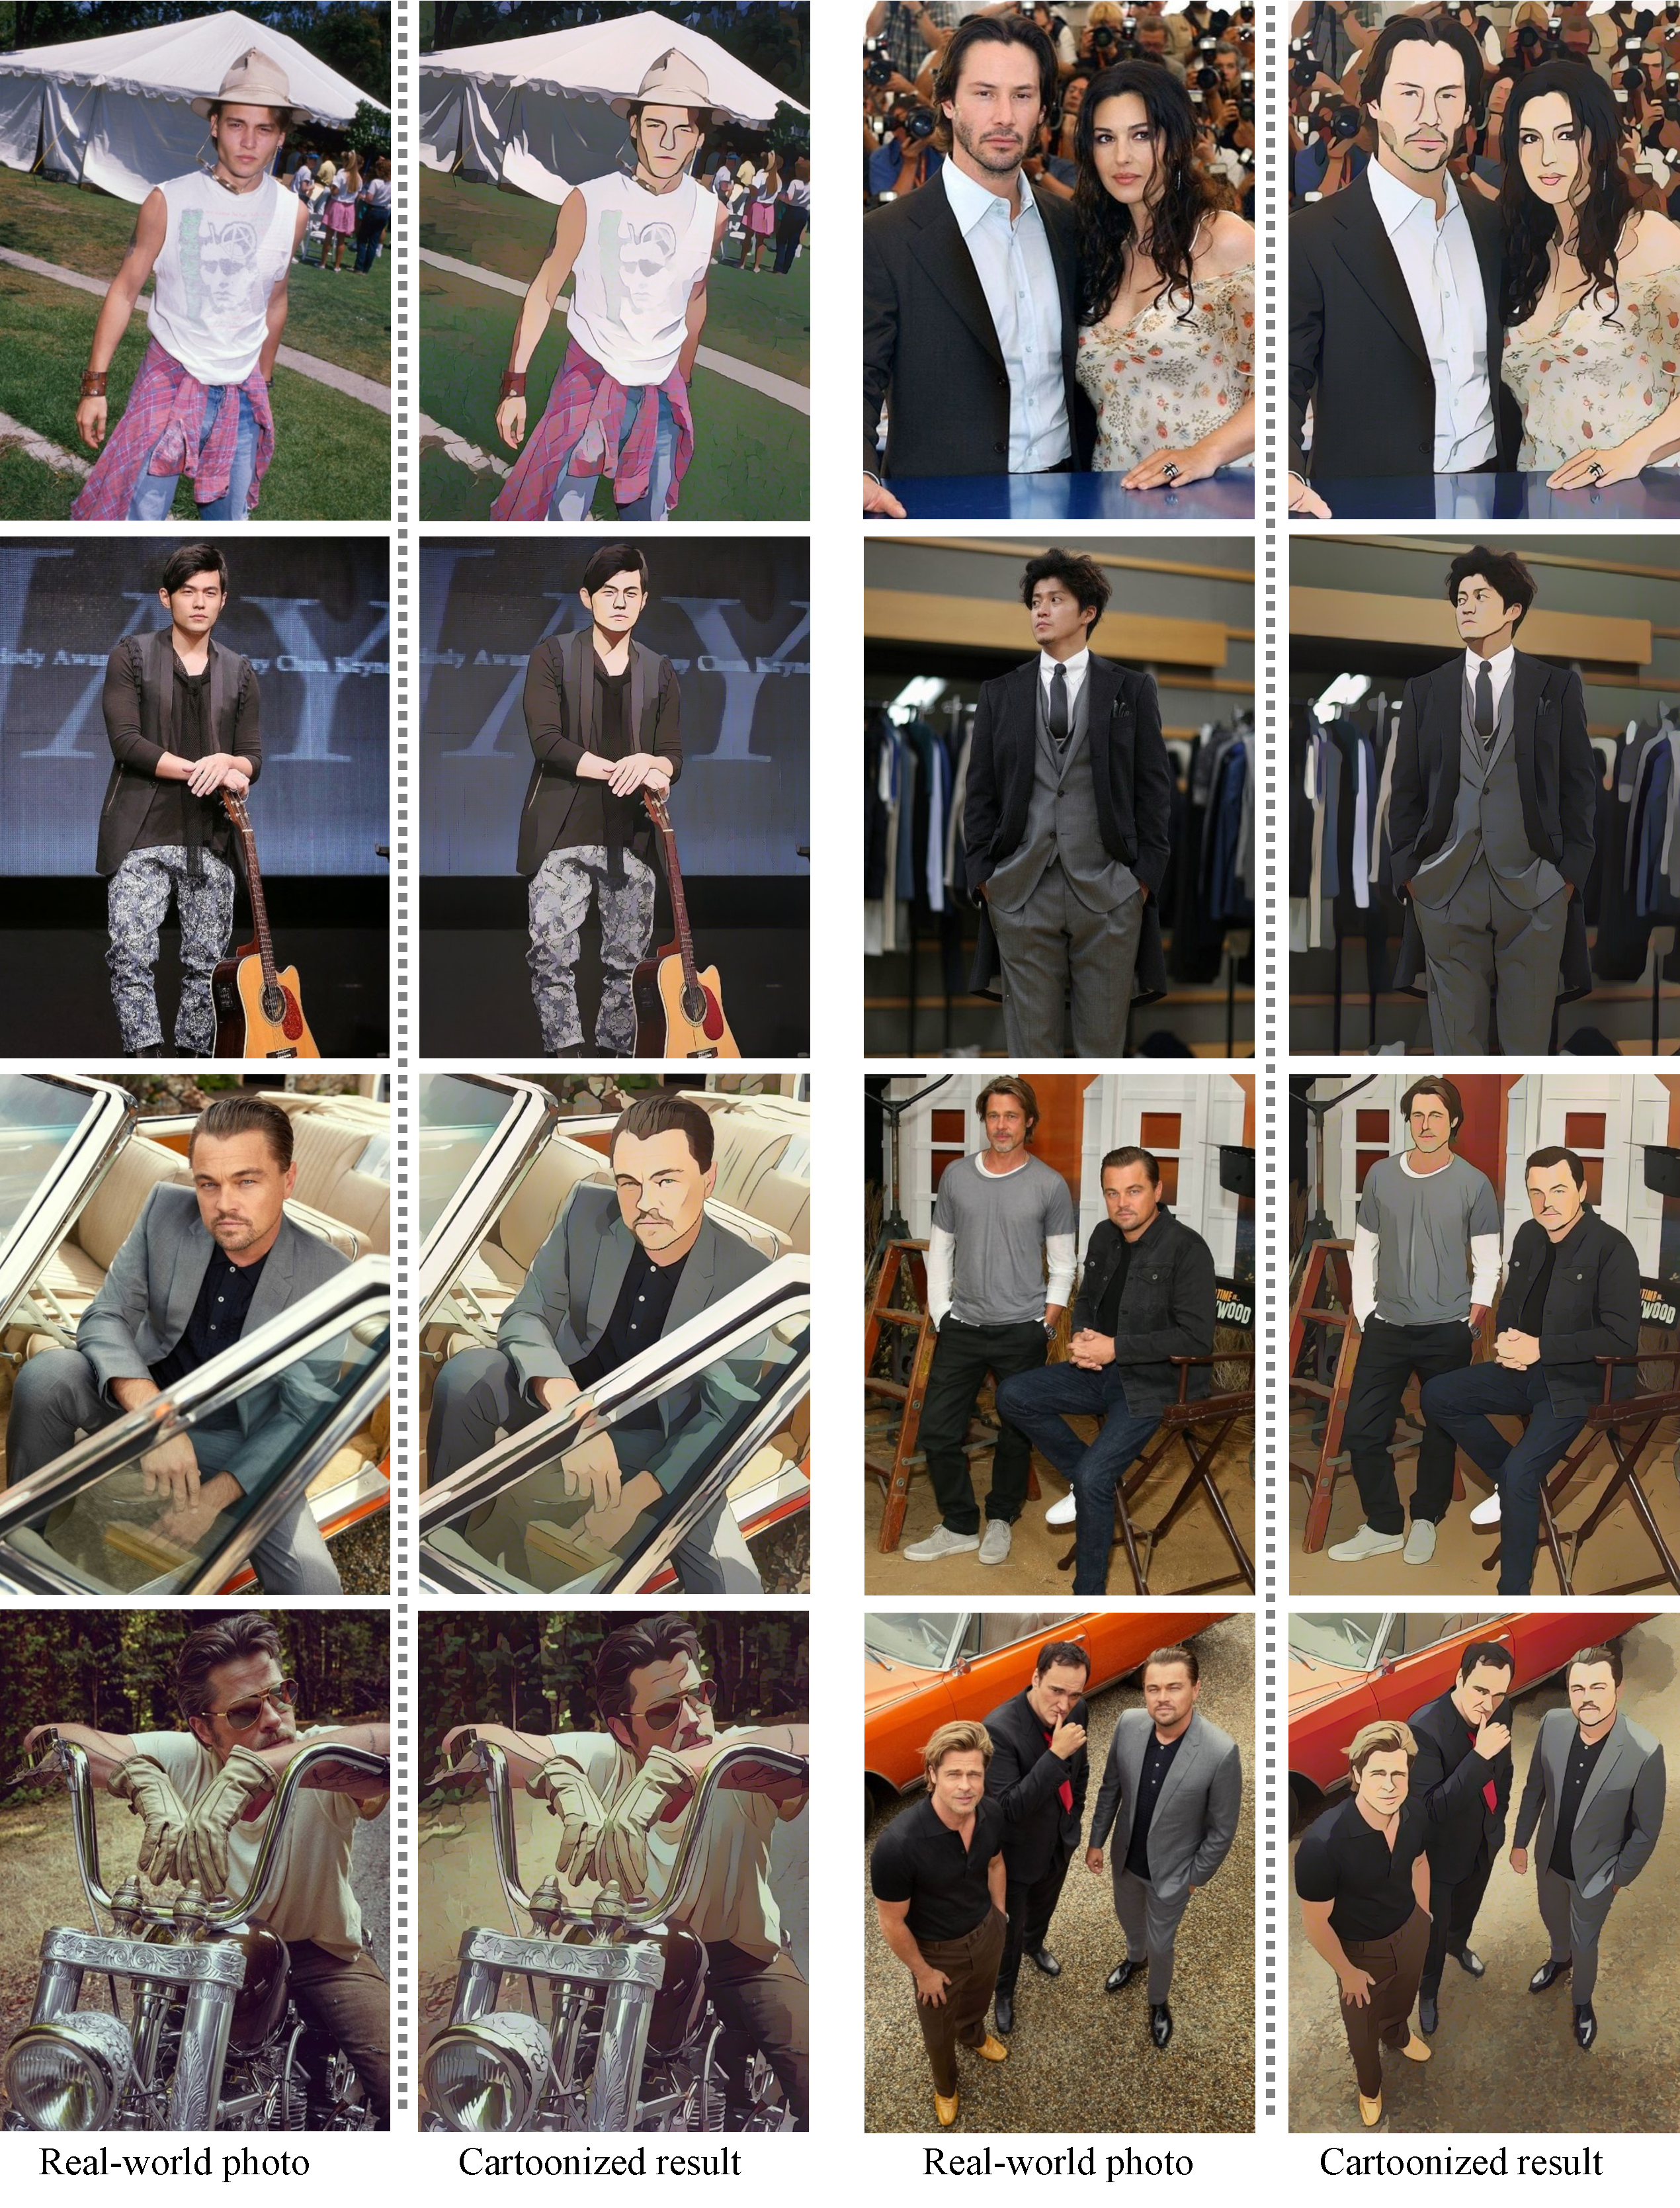
\includegraphics[width=\linewidth]{figures/person1.pdf}
\caption{Cartoonized male Celebrities.}
\label{fig:person1}
\vspace{-0.5em}
\end{figure*}

\begin{figure*}[b]
\vspace{-0.5em}
\centering
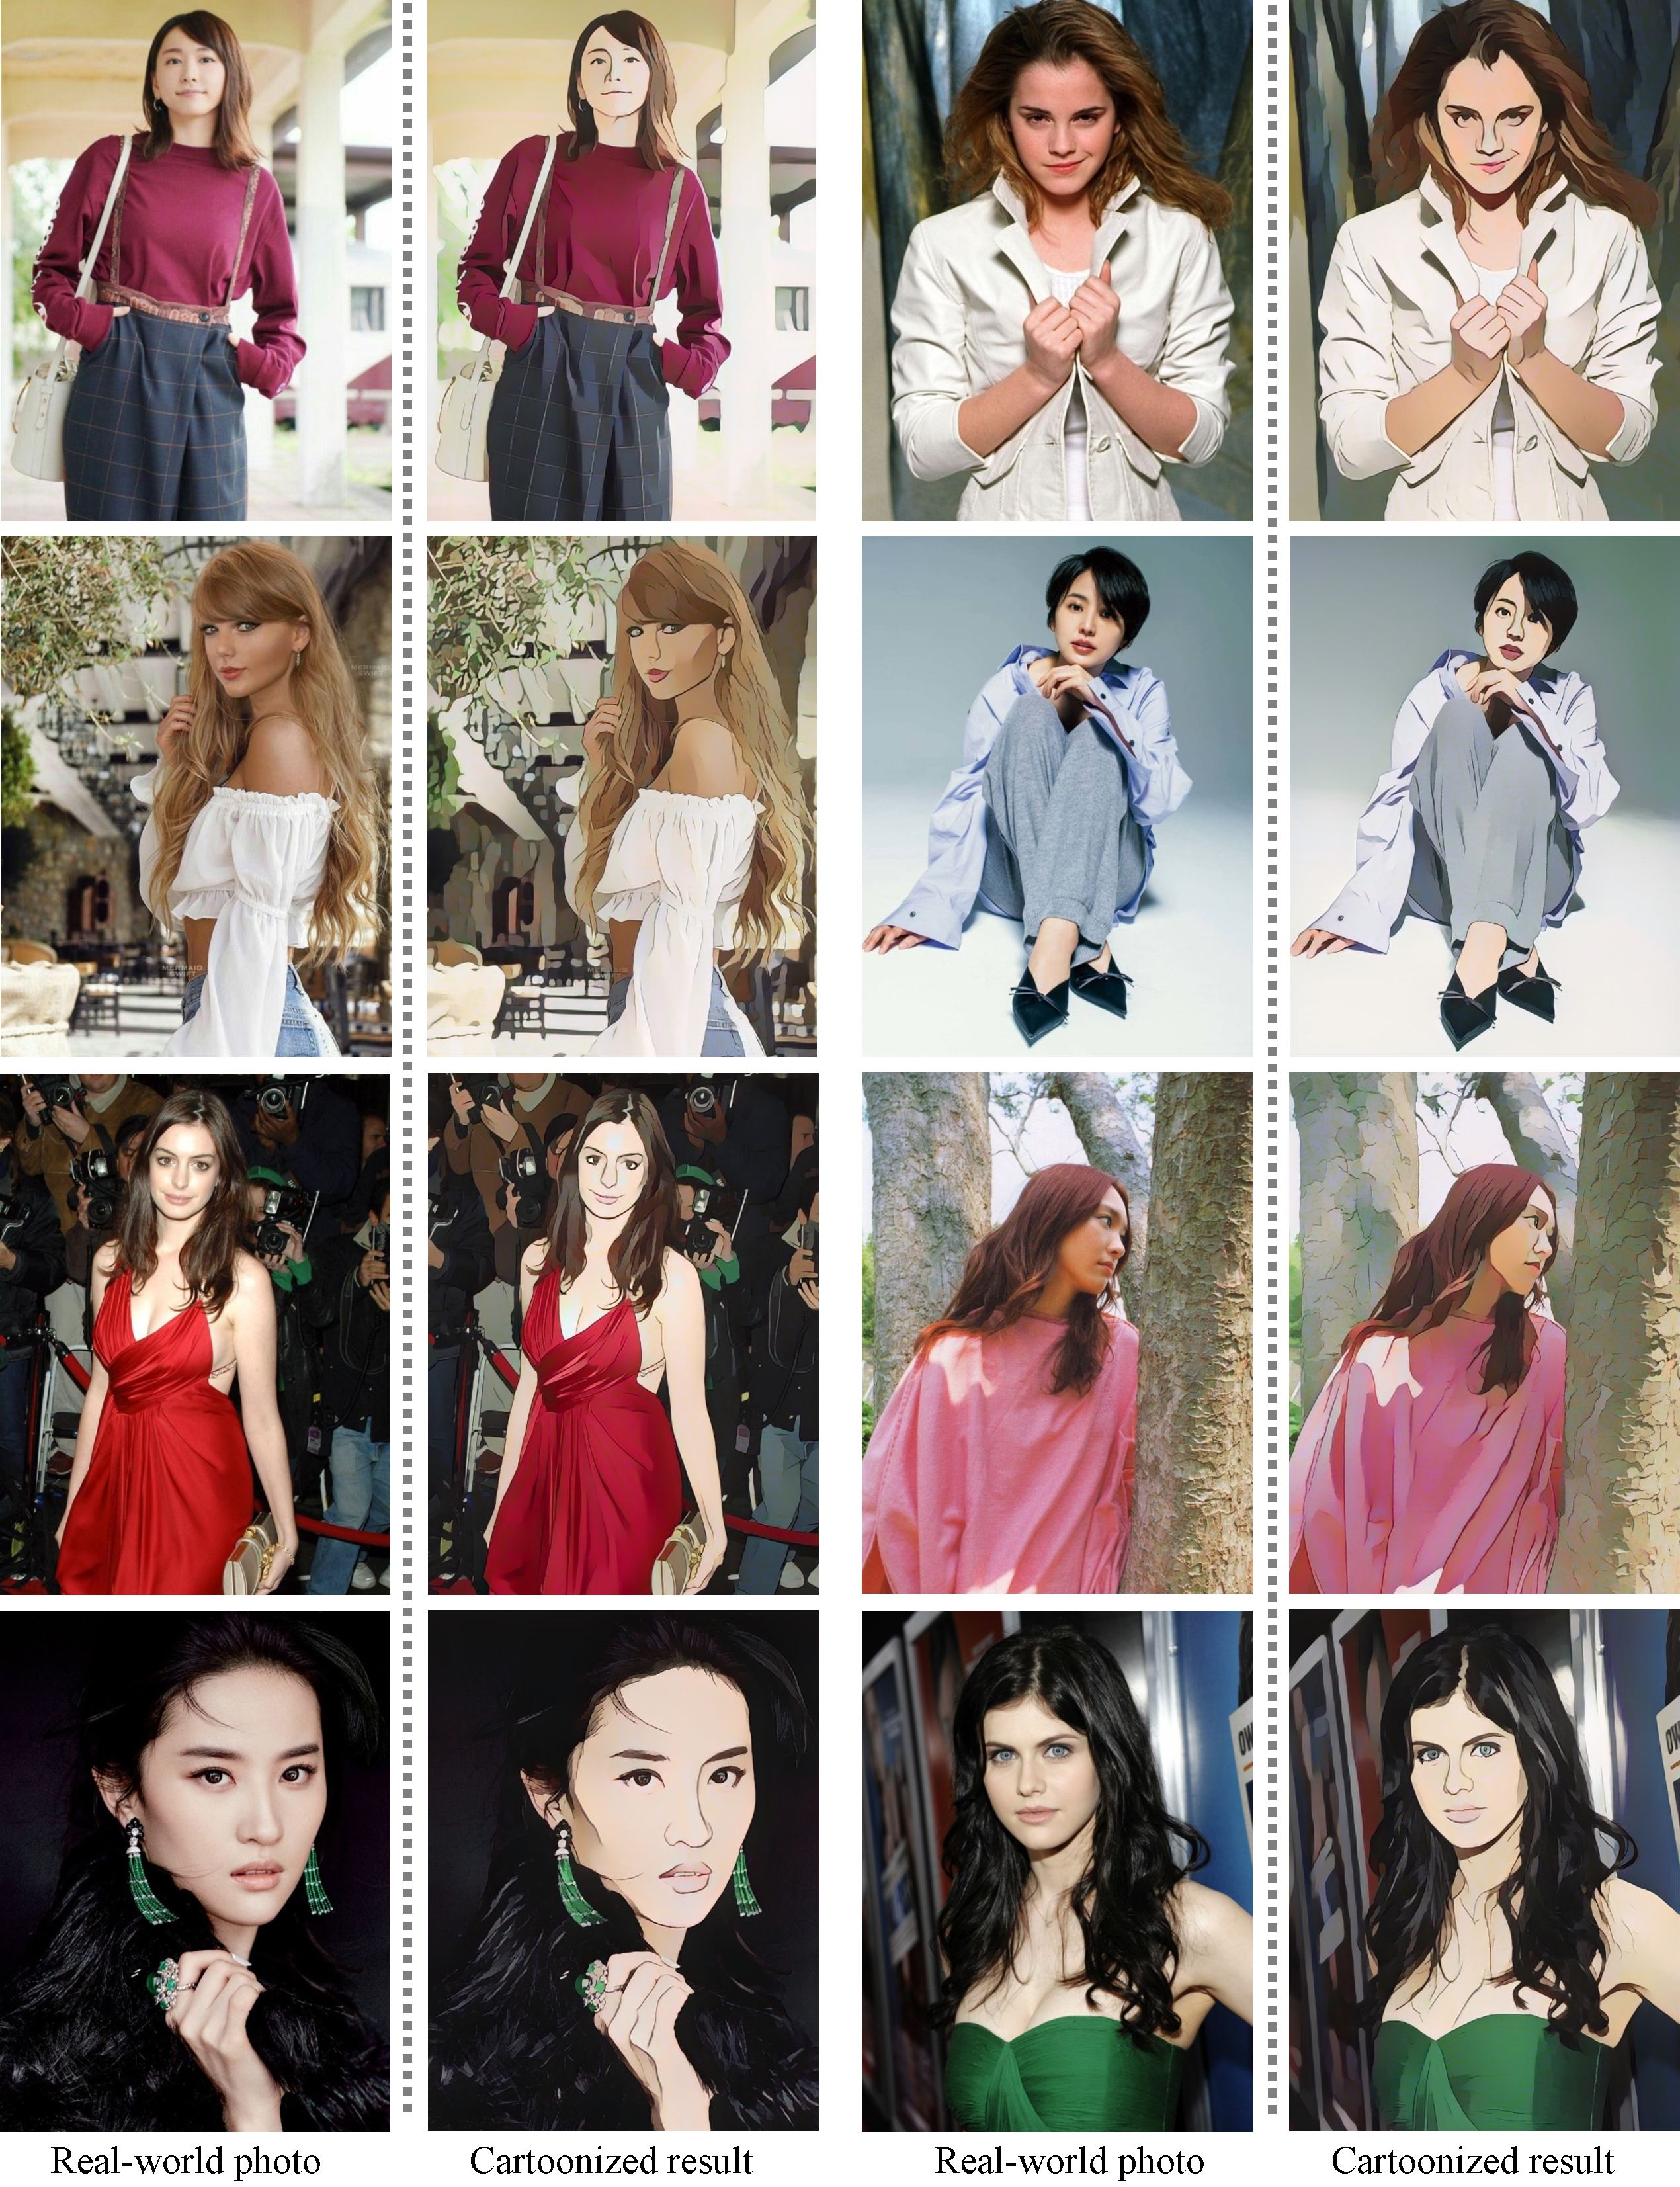
\includegraphics[width=\linewidth]{figures/person2.pdf}
\caption{Cartoonized female Celebrities.}
\label{fig:person2}
\vspace{-0.5em}
\end{figure*}

\begin{figure*}[b]
\vspace{-0.5em}
\centering
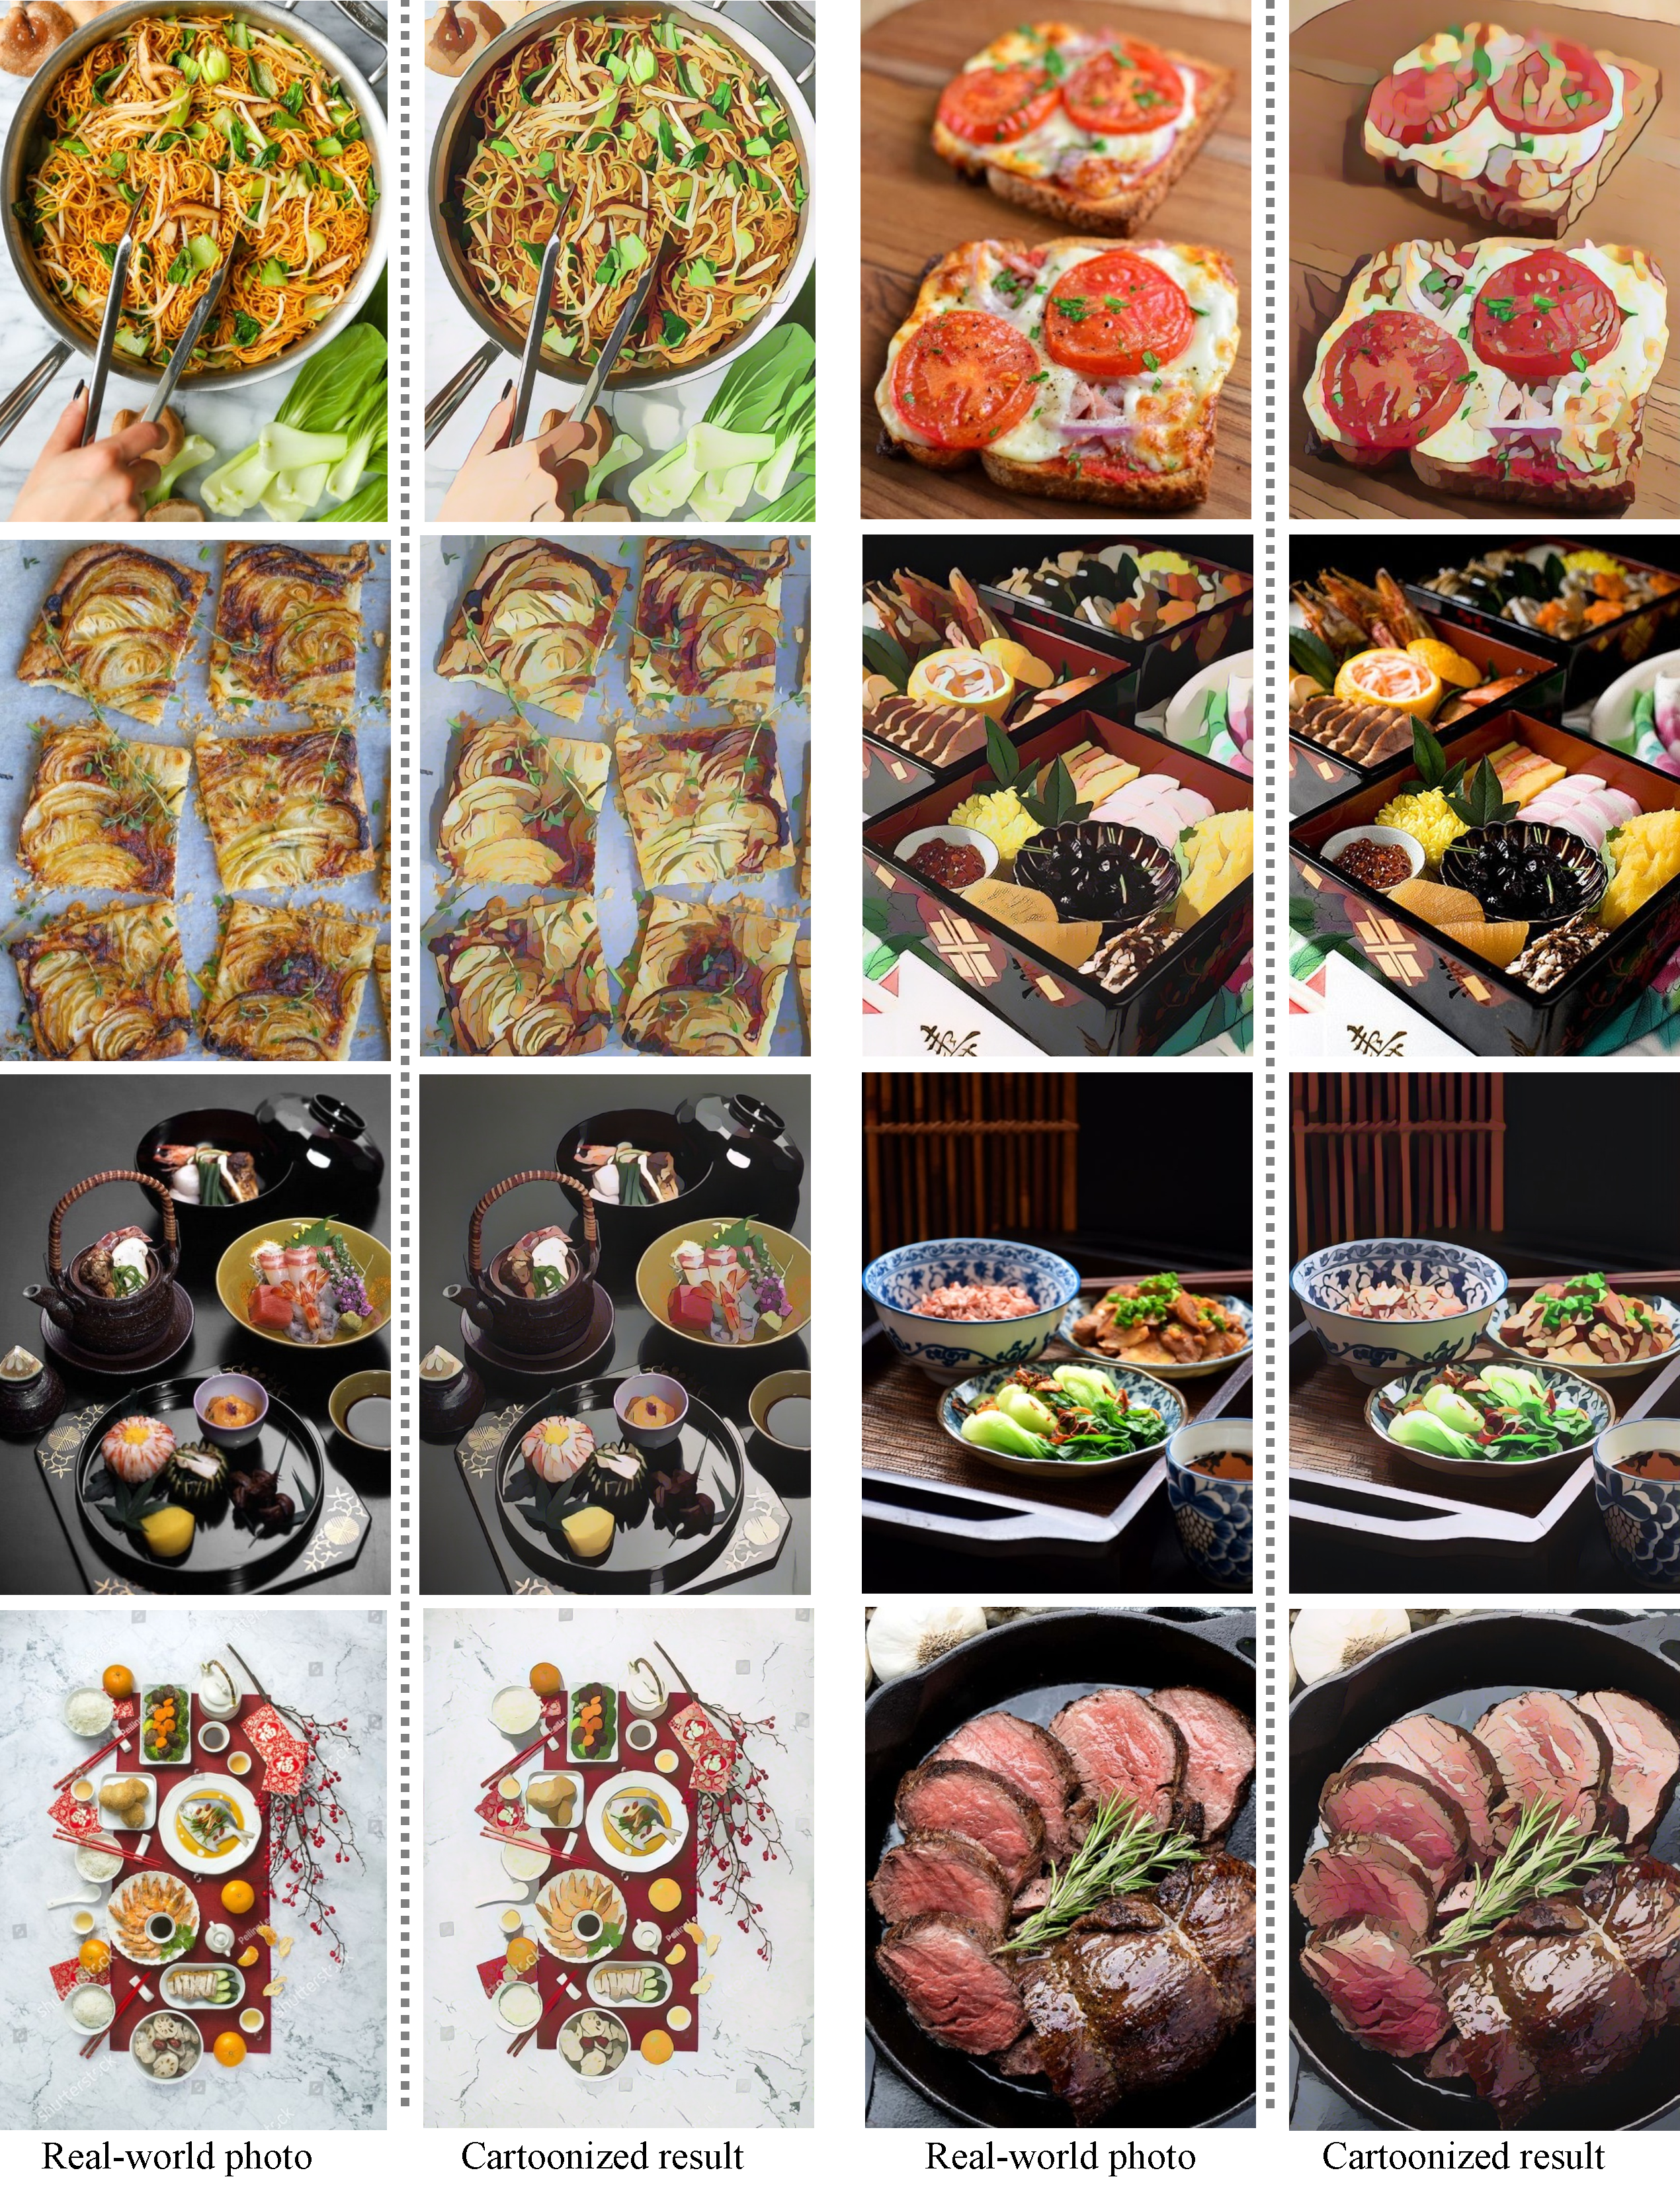
\includegraphics[width=\linewidth]{figures/food.pdf}
\caption{Cartoonized food.}
\label{fig:food}
%\vspace{-1em}
\end{figure*}

\begin{figure*}[b]
%\vspace{-1em}
\centering
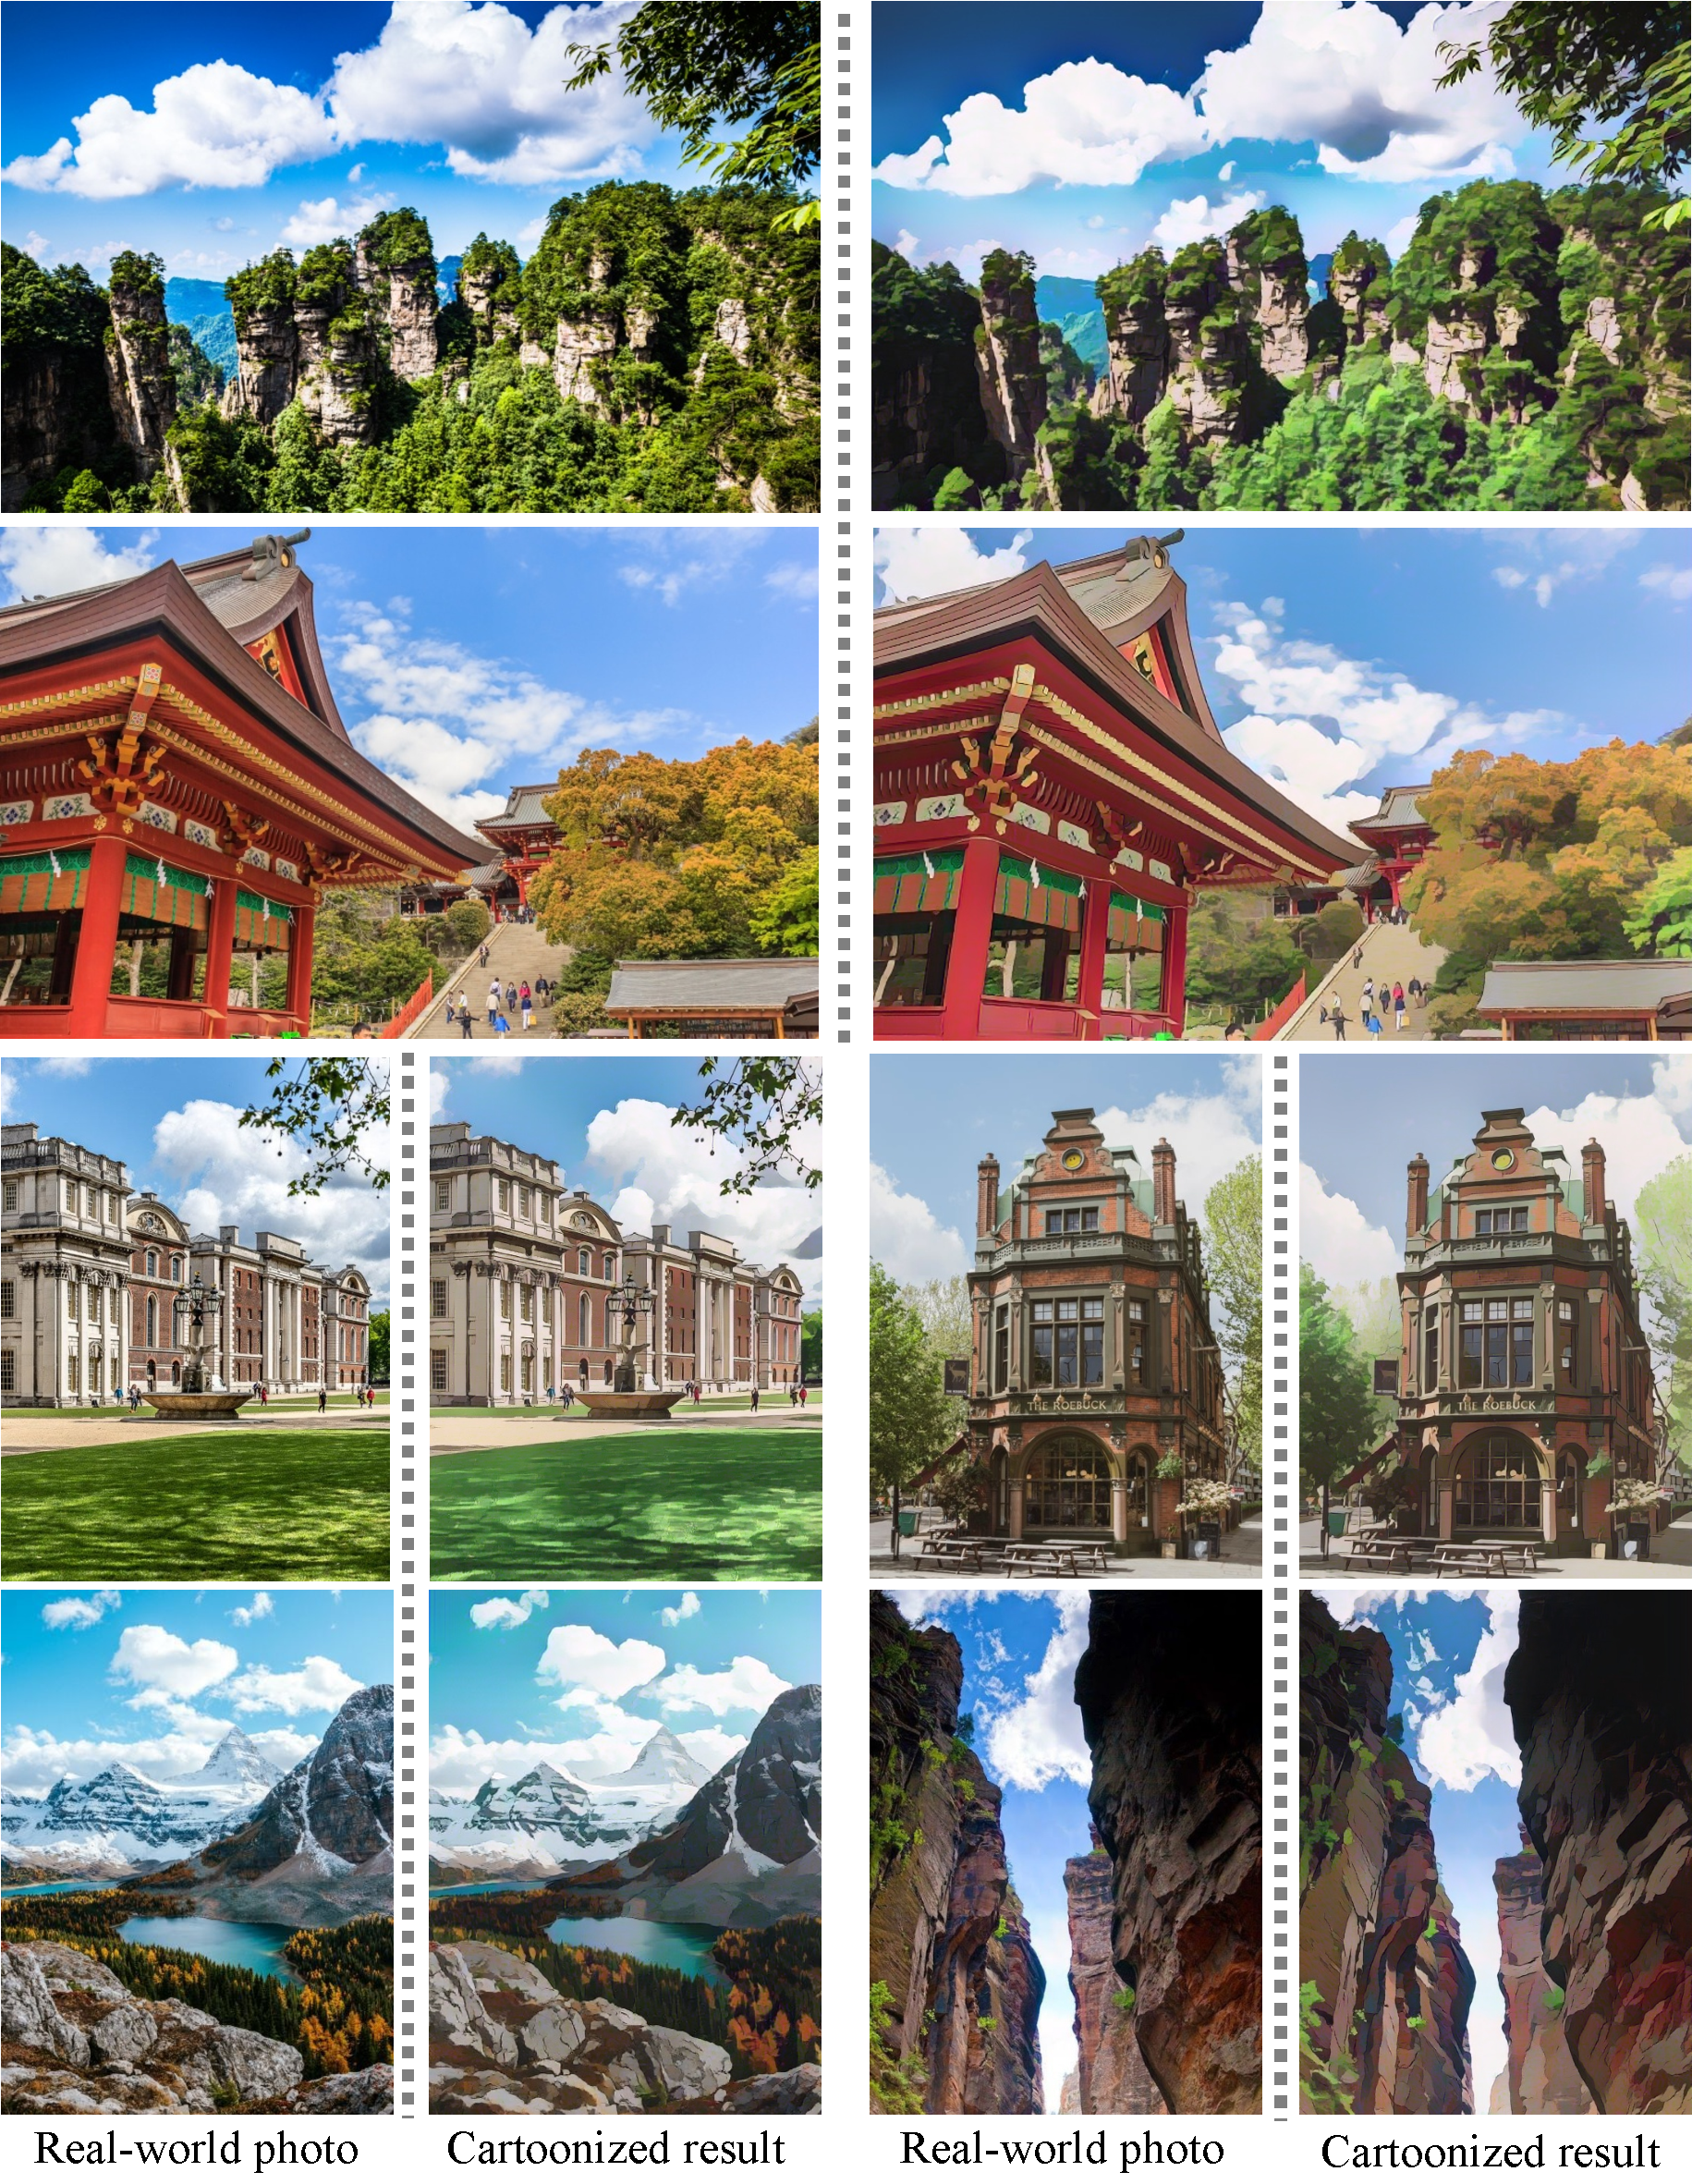
\includegraphics[width=\linewidth]{figures/scenery1.pdf}
\caption{Cartoonized scenery.}
\label{fig:scenery1}
%\vspace{-1em}
\end{figure*}

\begin{figure*}[b]
%\vspace{-1em}
\centering
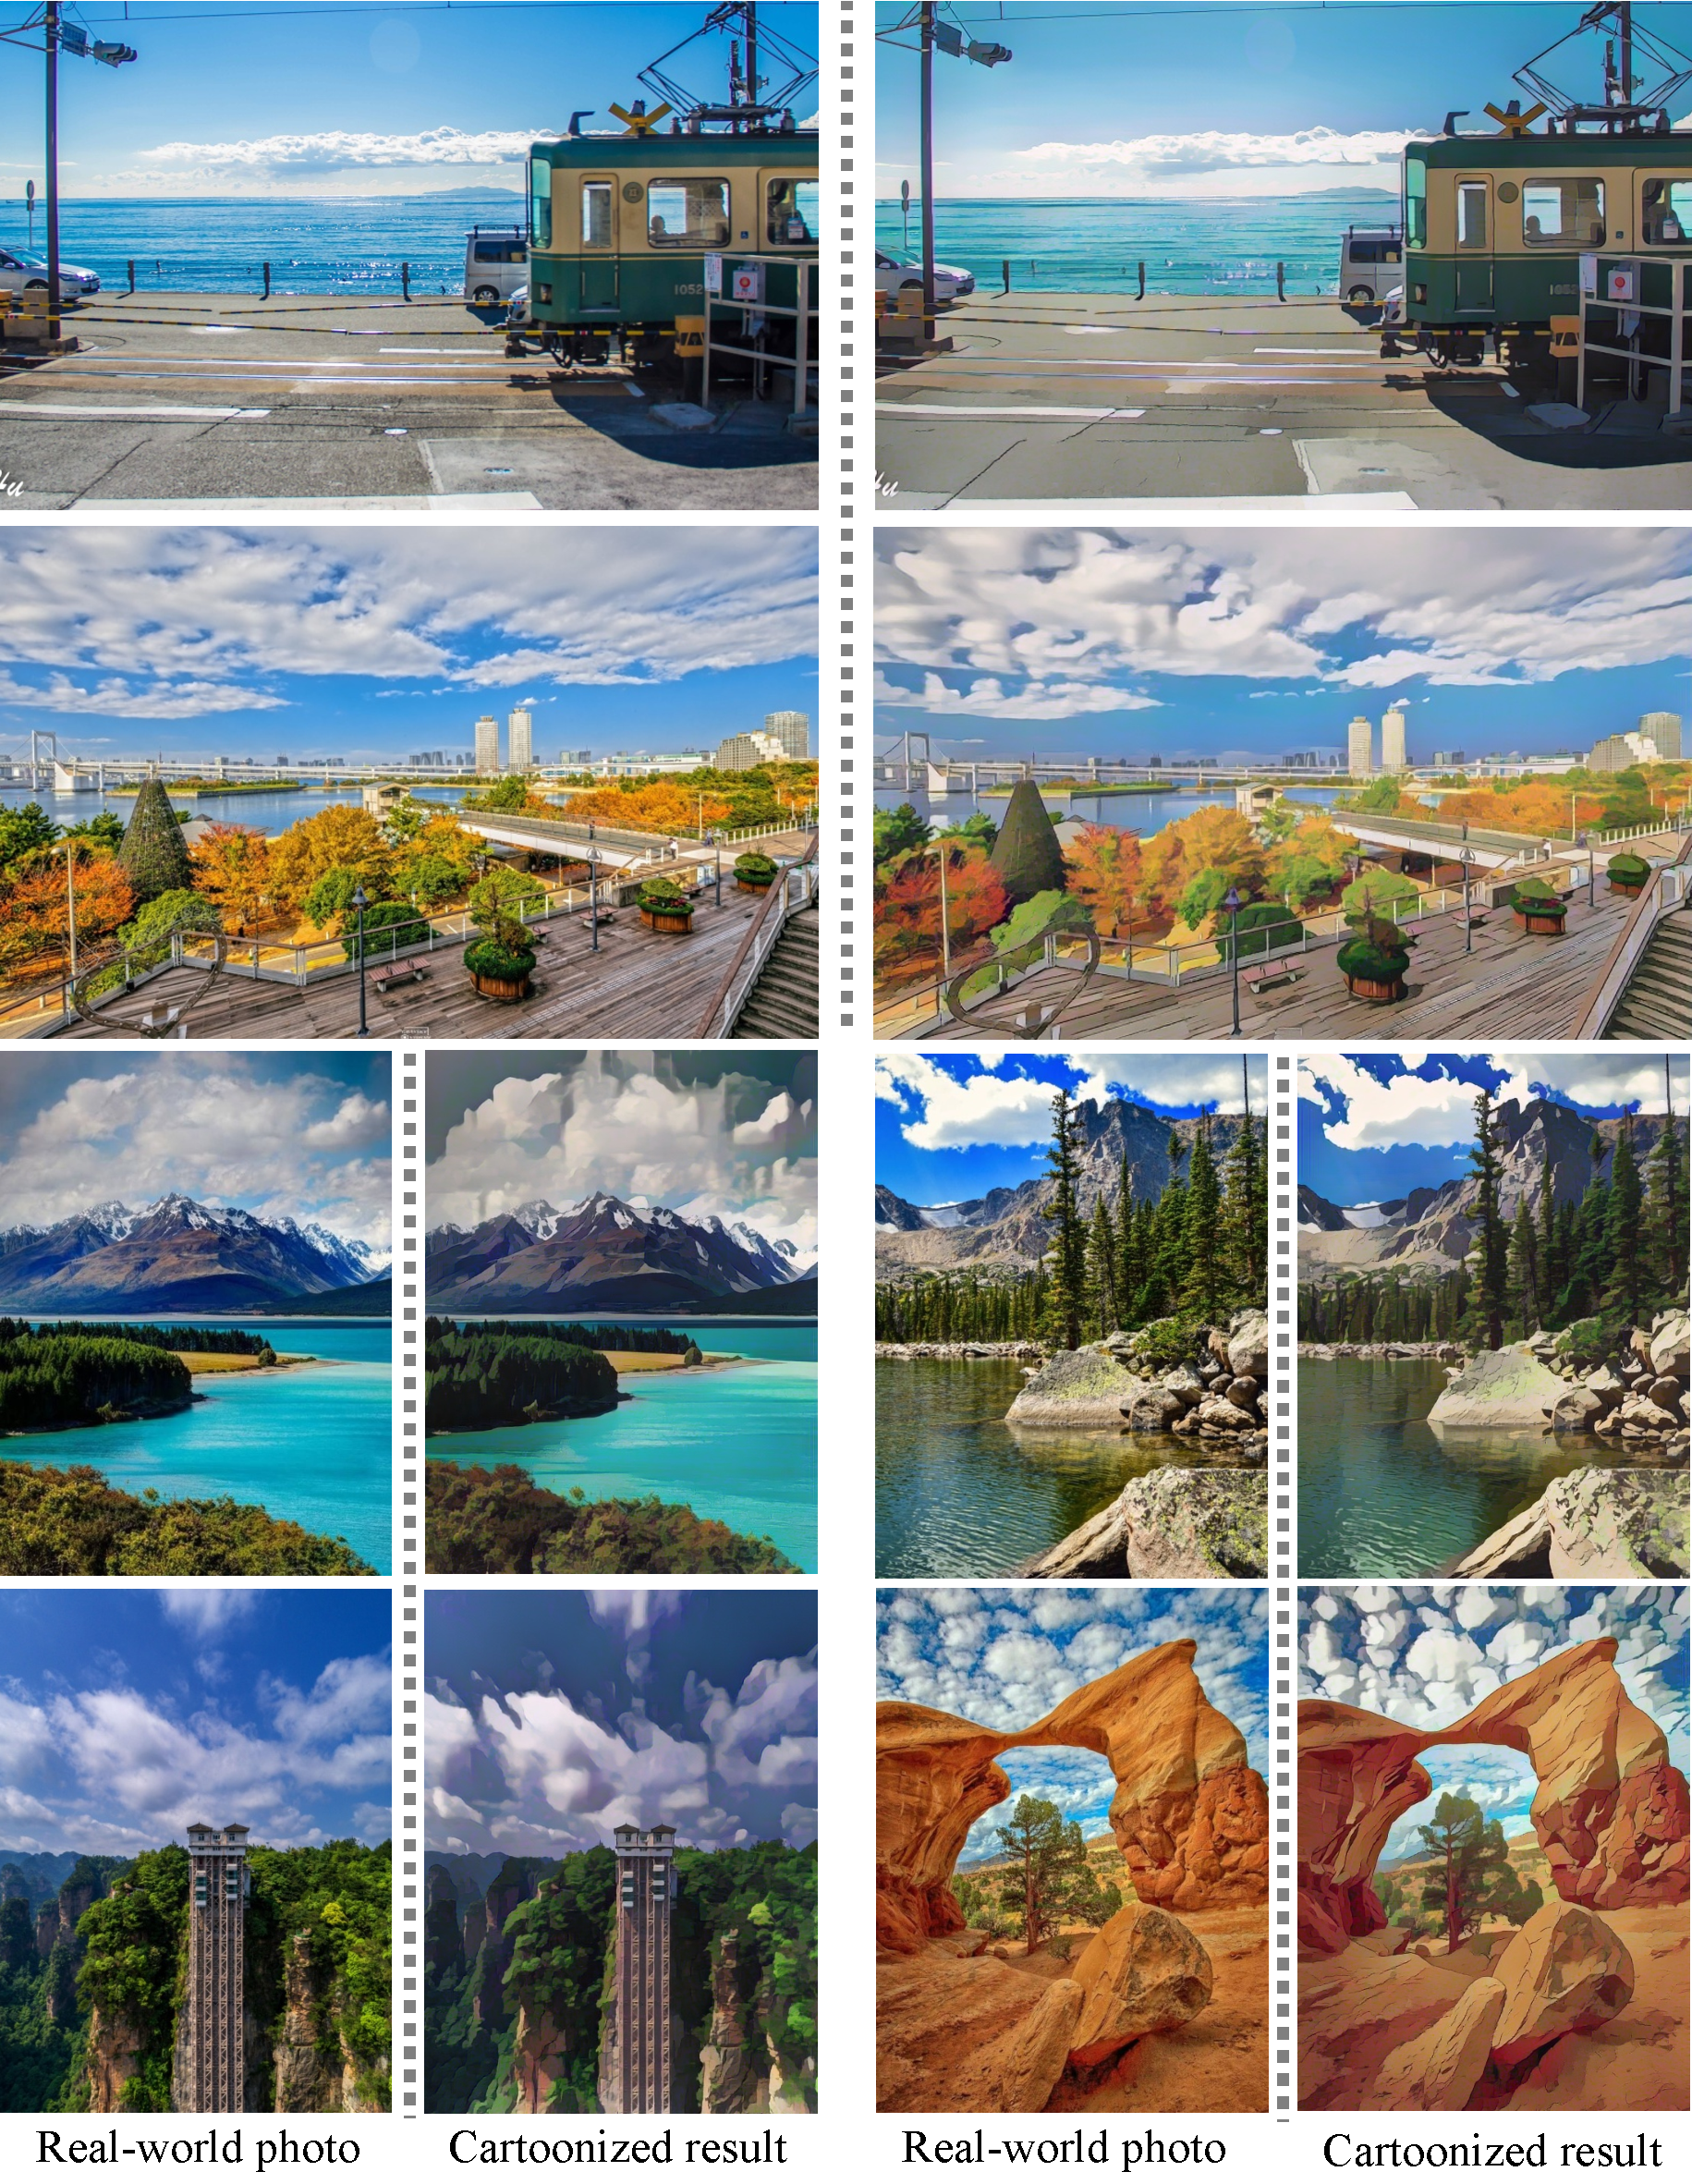
\includegraphics[width=\linewidth]{figures/scenery2.pdf}
\caption{Cartoonized scenery.}
\label{fig:scenery2}
%\vspace{-1em}
\end{figure*}

\begin{figure*}[b]
\vspace{-0.5em}
\centering
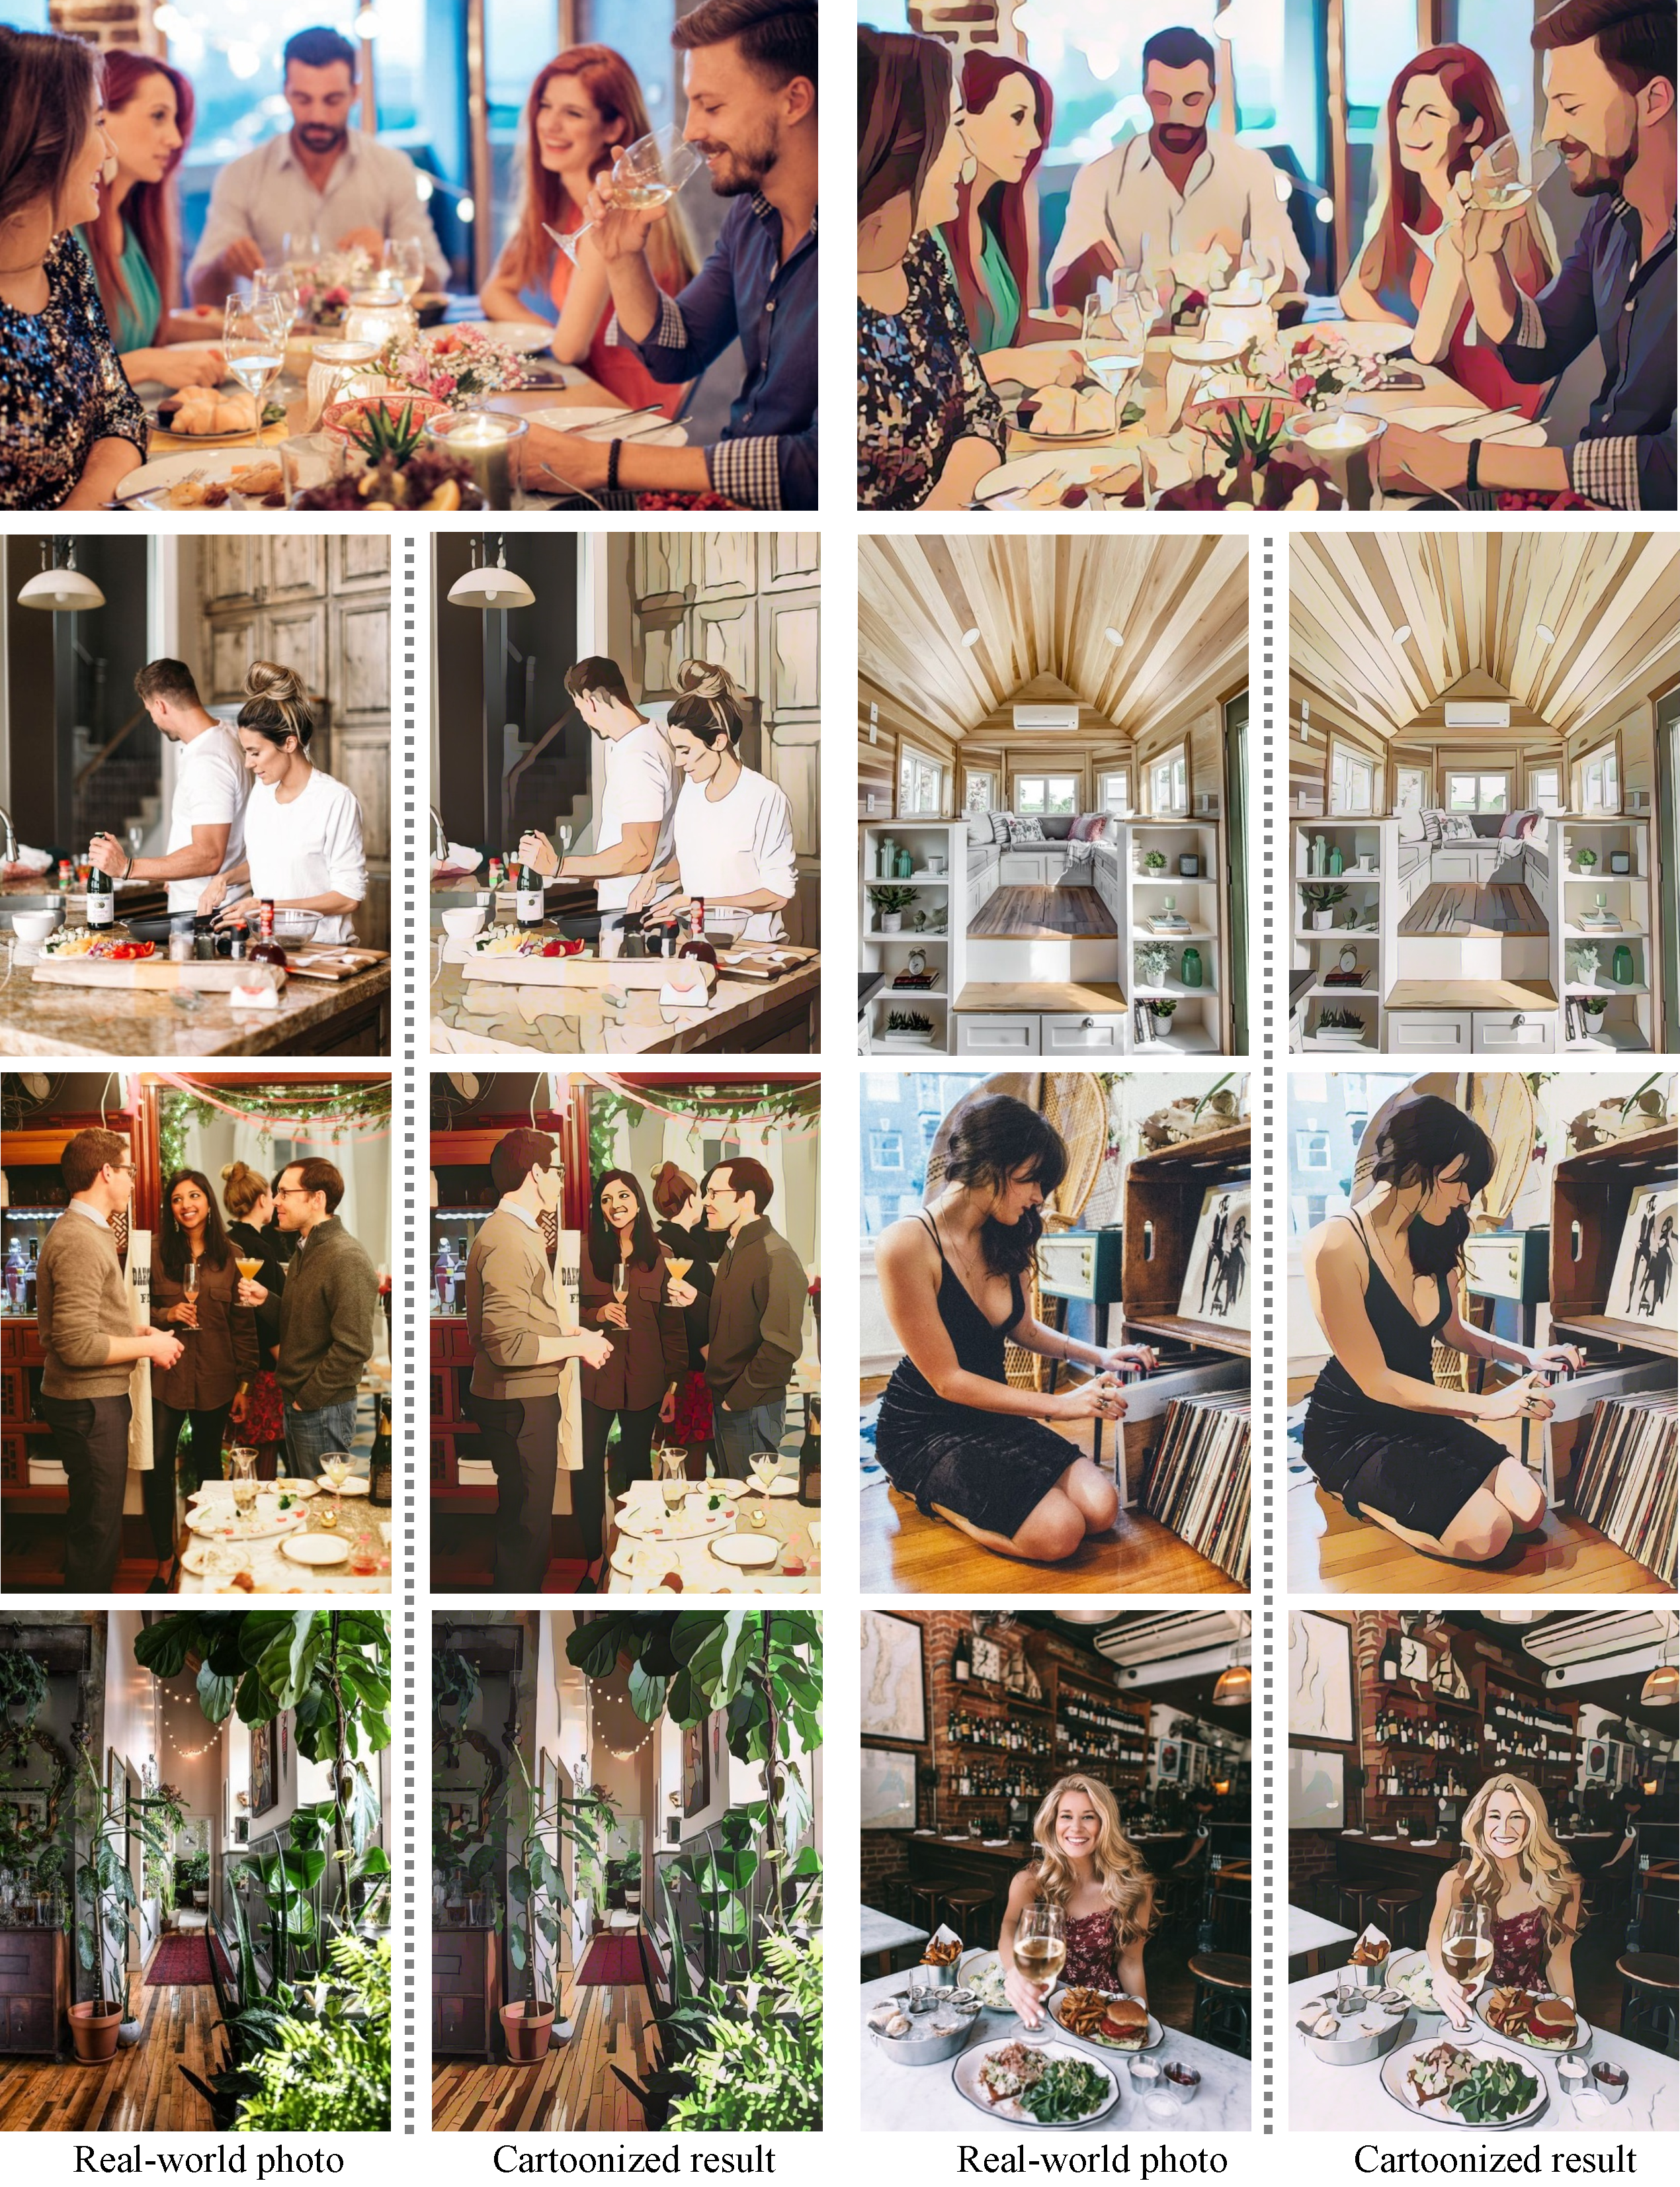
\includegraphics[width=\linewidth]{figures/home.pdf}
\caption{Cartoonized indoor scenes.}
\label{fig:home}
\end{figure*}

\begin{figure*}[b]
\vspace{-0.5em}
\centering
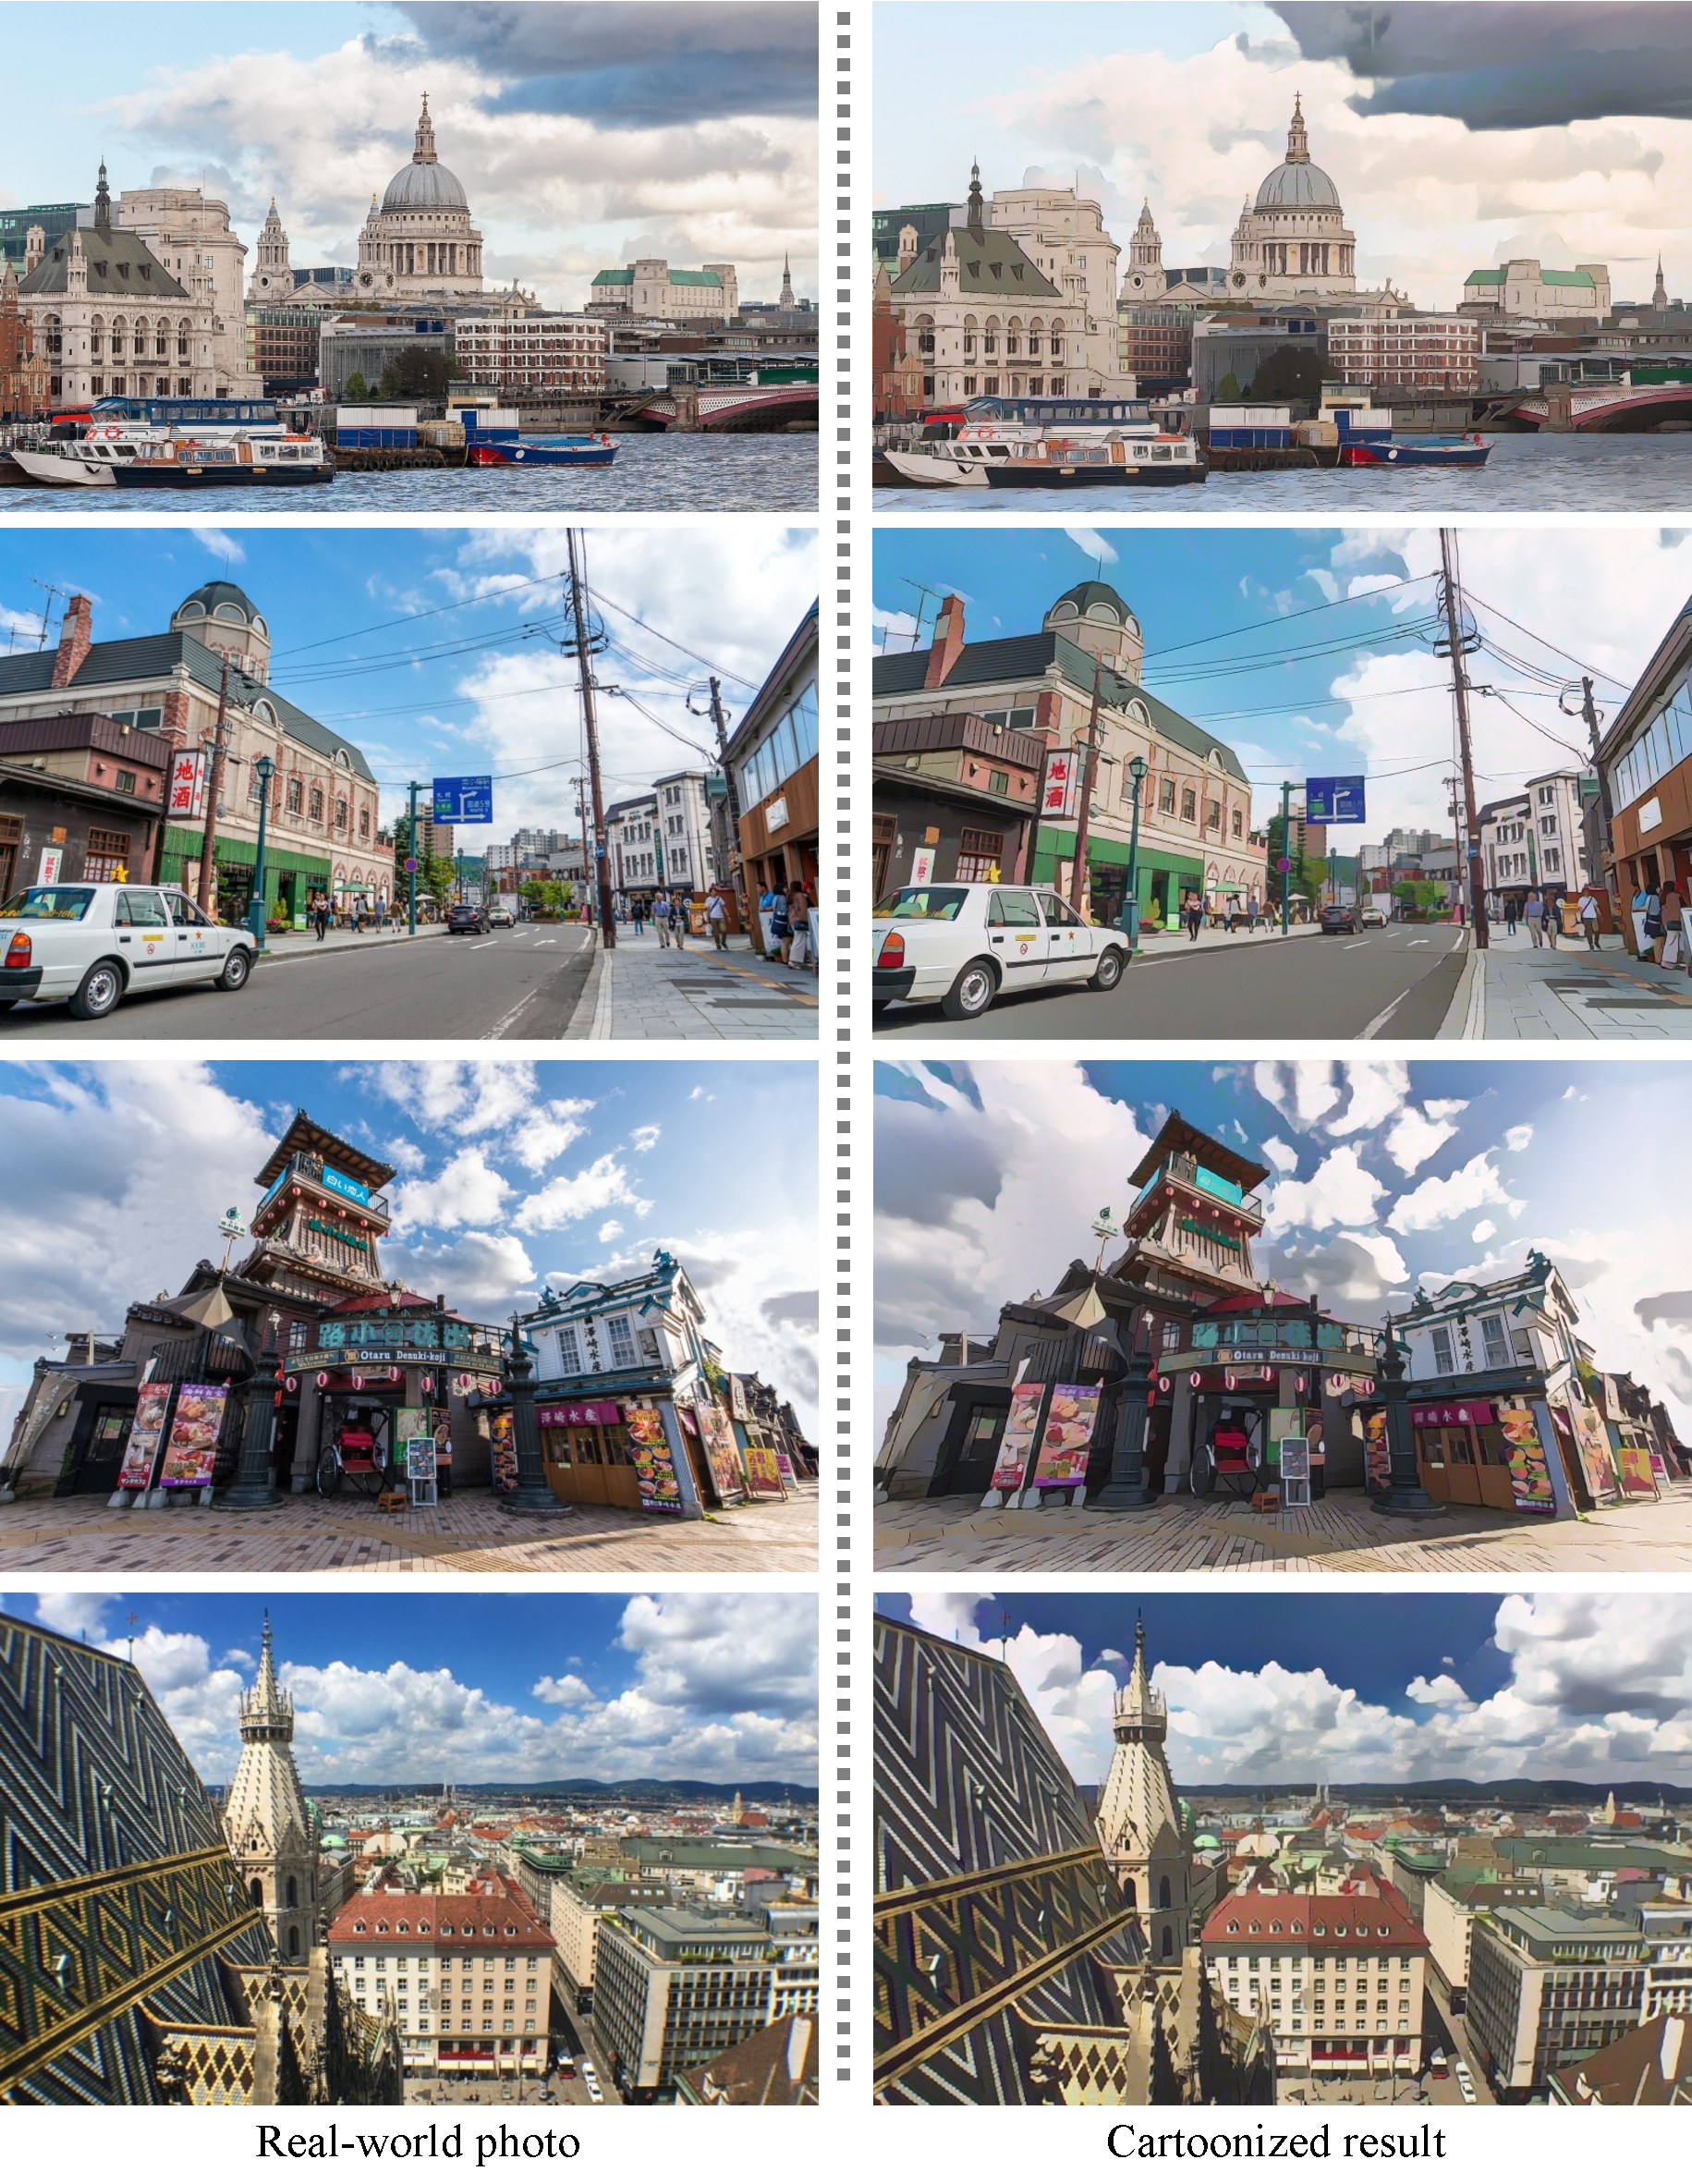
\includegraphics[width=\linewidth]{figures/city1.pdf}
\caption{Cartoonized city scenes.}
\label{fig:city1}
\end{figure*}

\begin{figure*}[b]
\vspace{-0.5em}
\centering
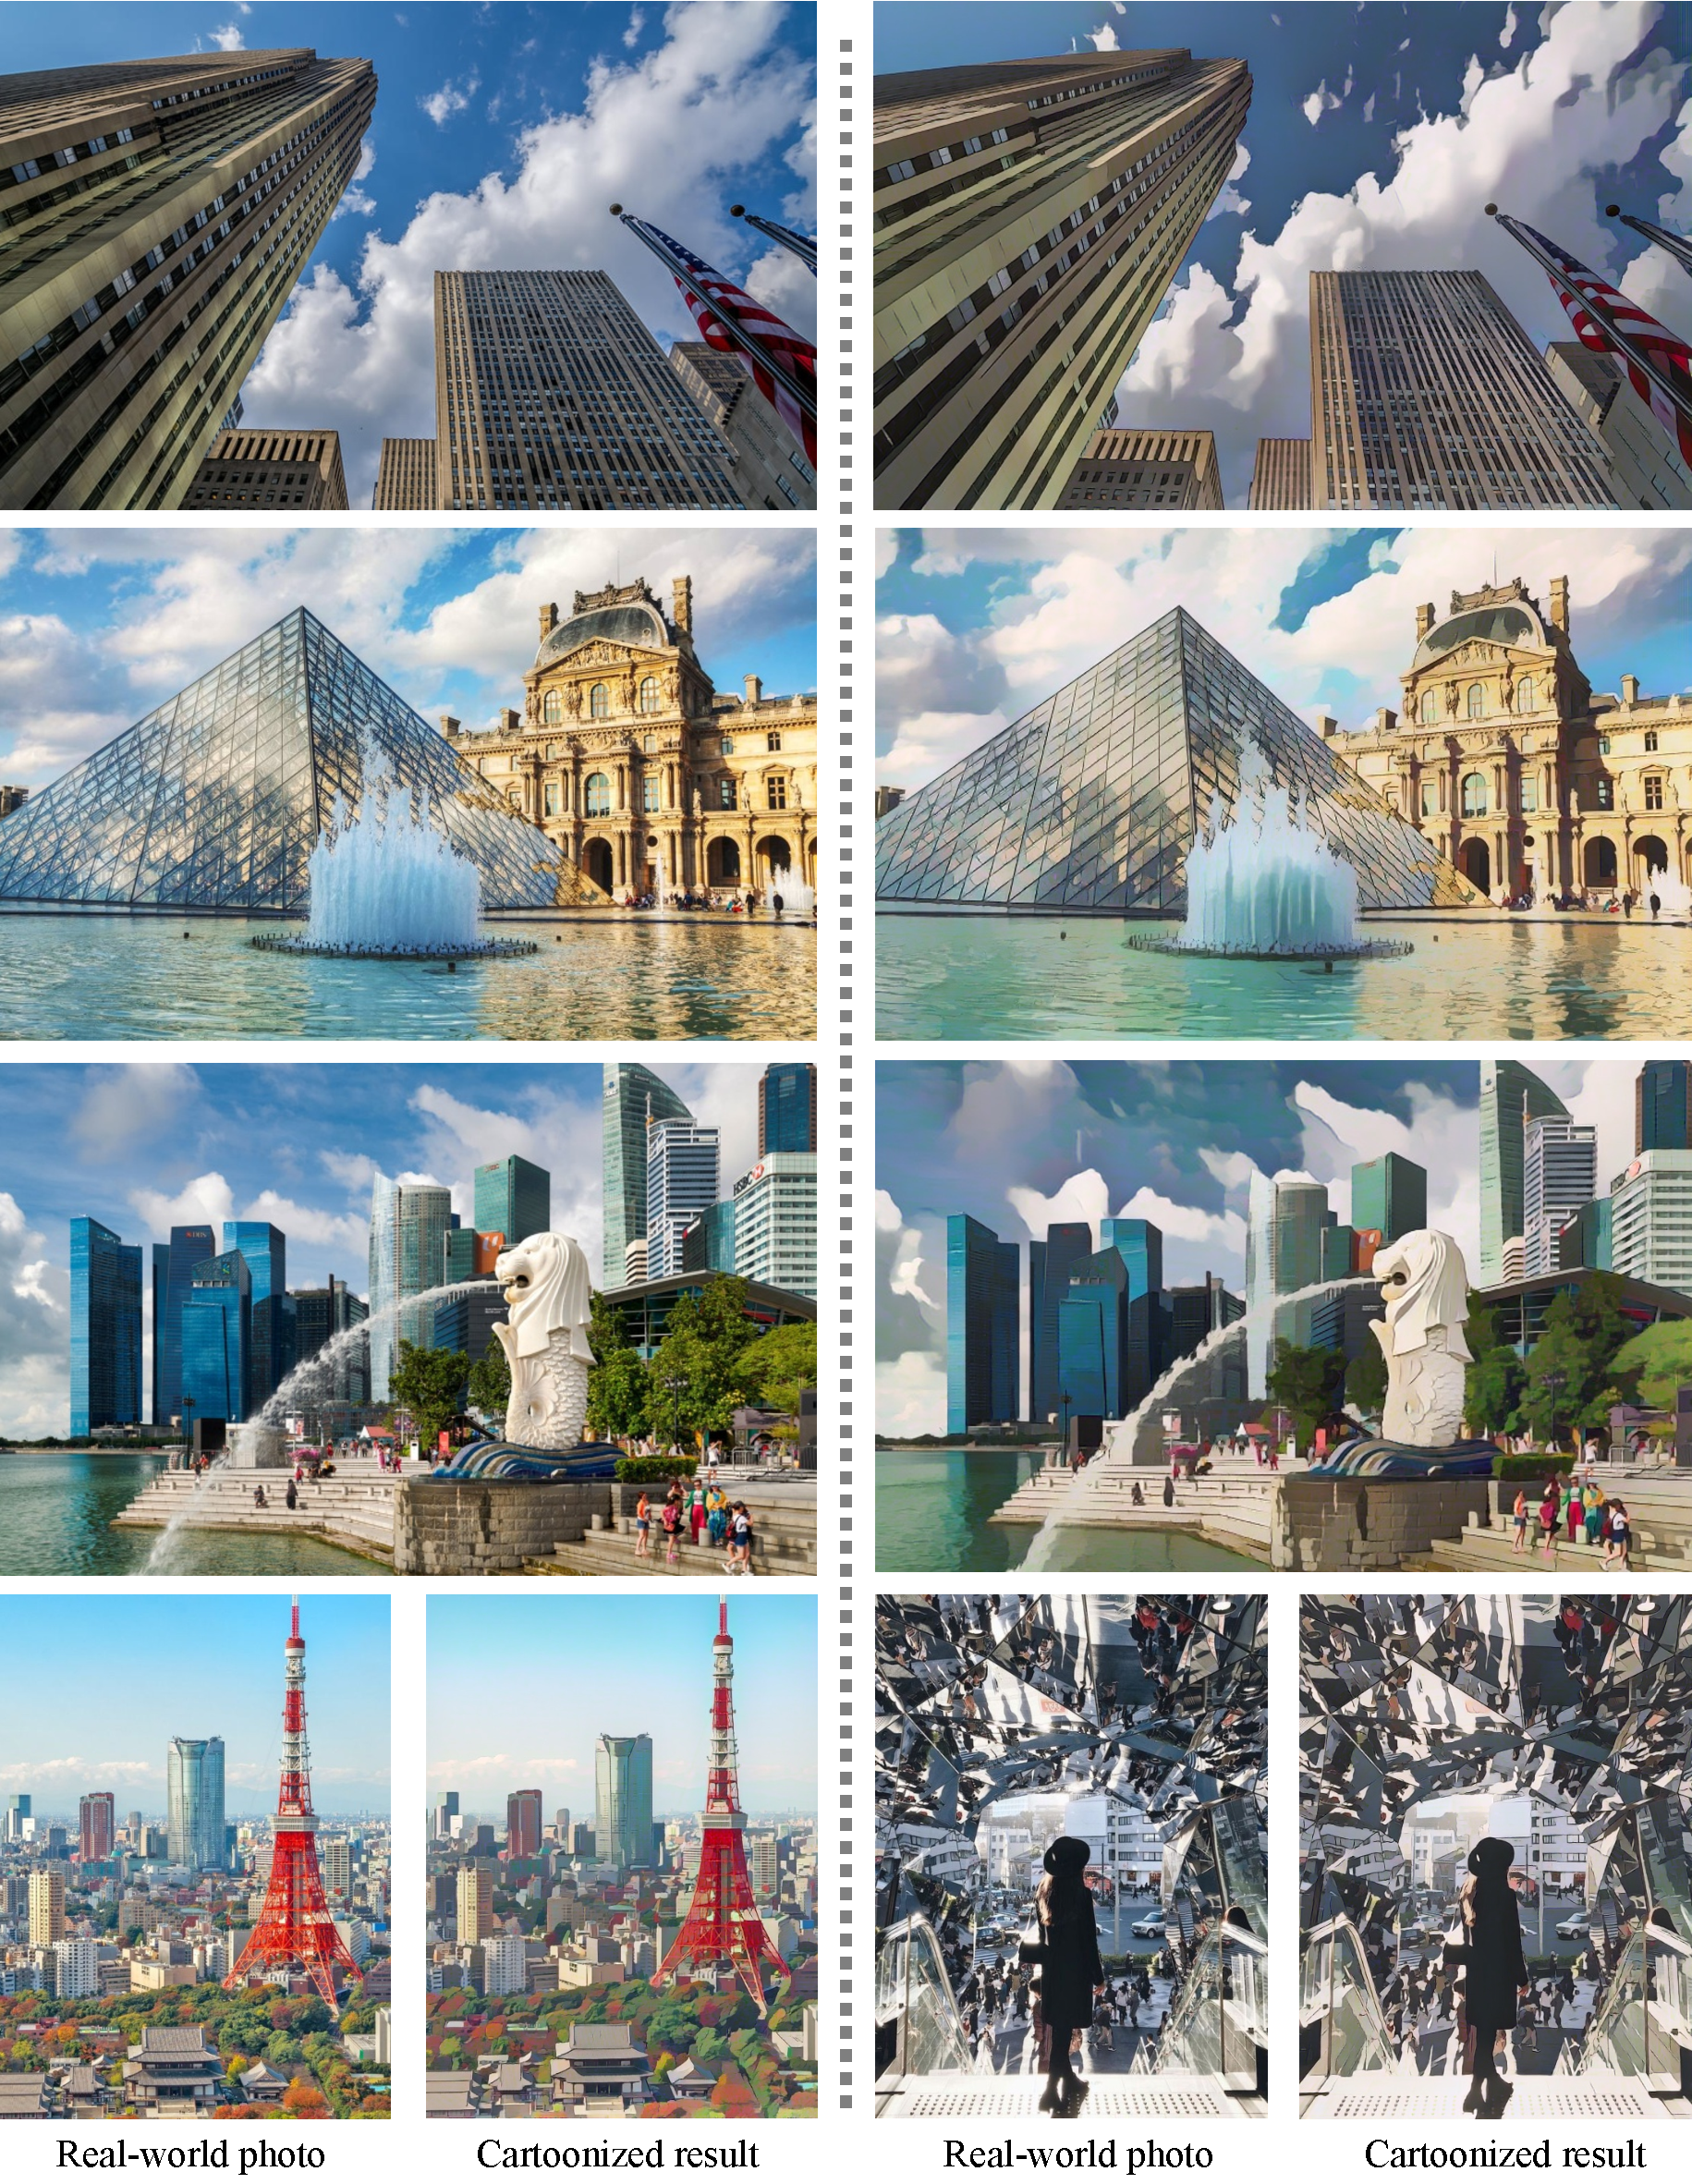
\includegraphics[width=\linewidth]{figures/city2.pdf}
\caption{Cartoonized city scenes.}
\label{fig:city2}
\end{figure*}

\begin{figure*}[b]
\vspace{-0.5em}
\centering
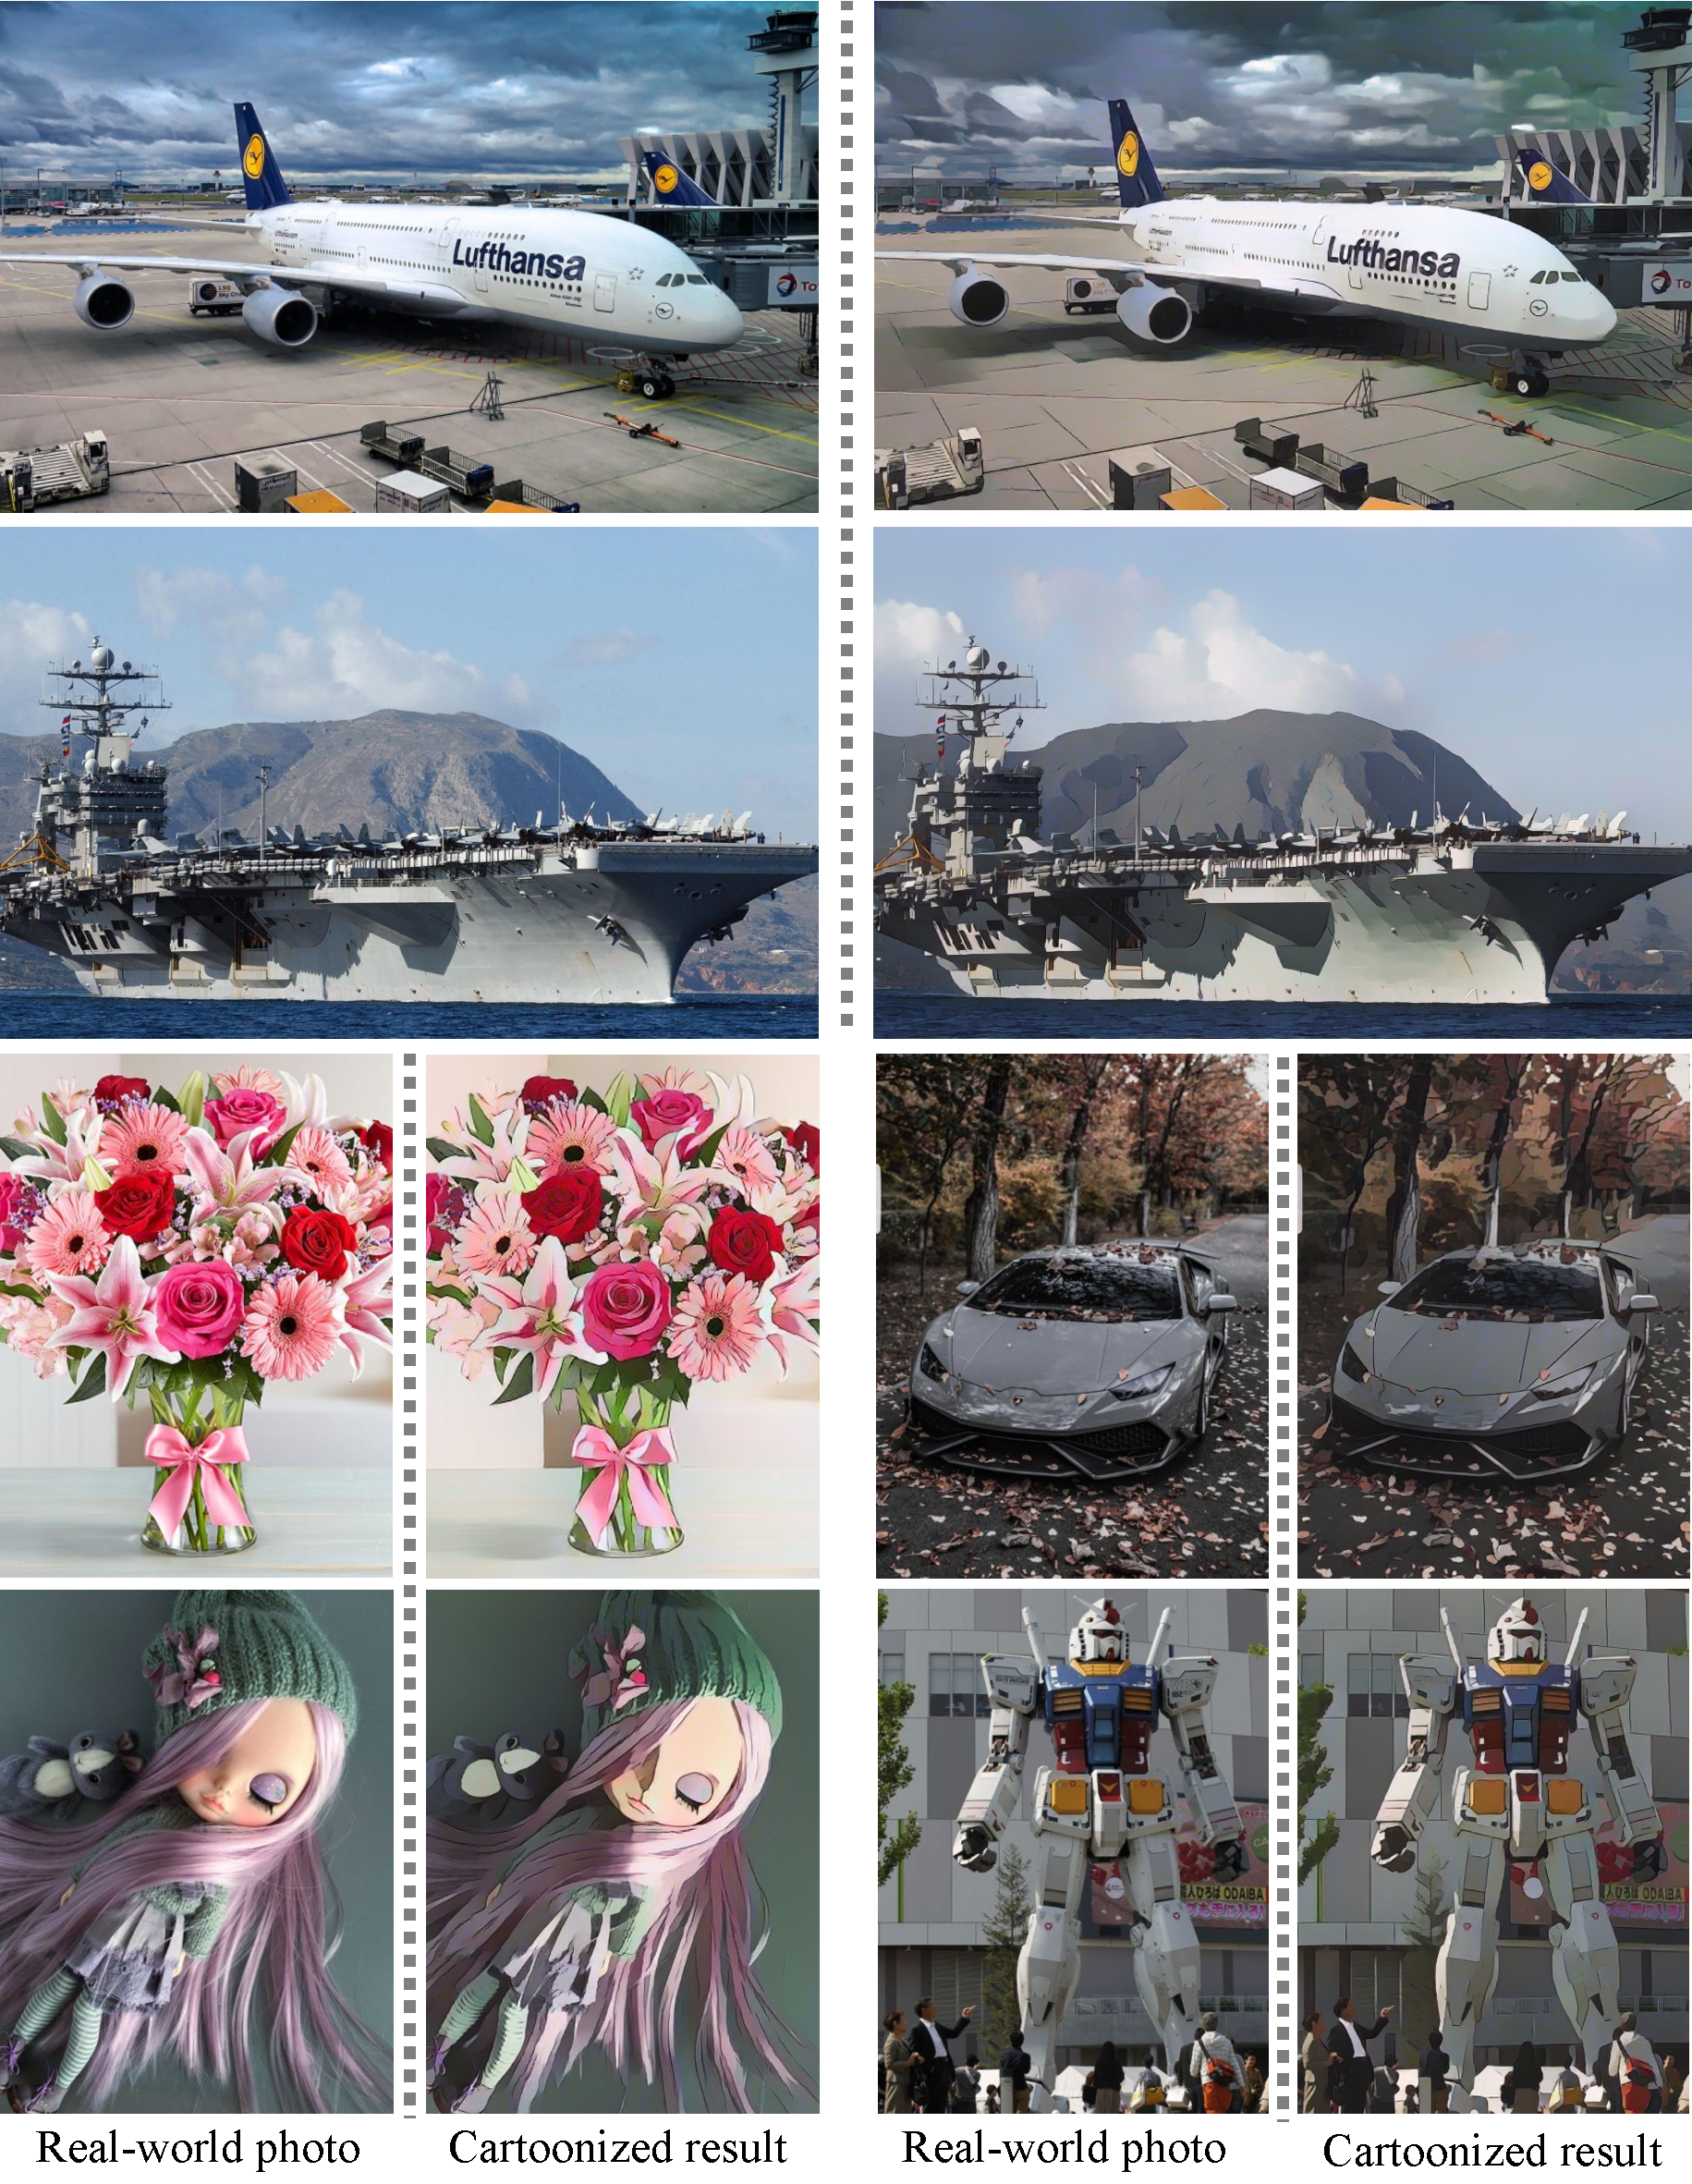
\includegraphics[width=\linewidth]{figures/object.pdf}
\caption{Cartoonized different objects.}
\label{fig:object}
\end{figure*}

\begin{figure*}[htb]
\centering
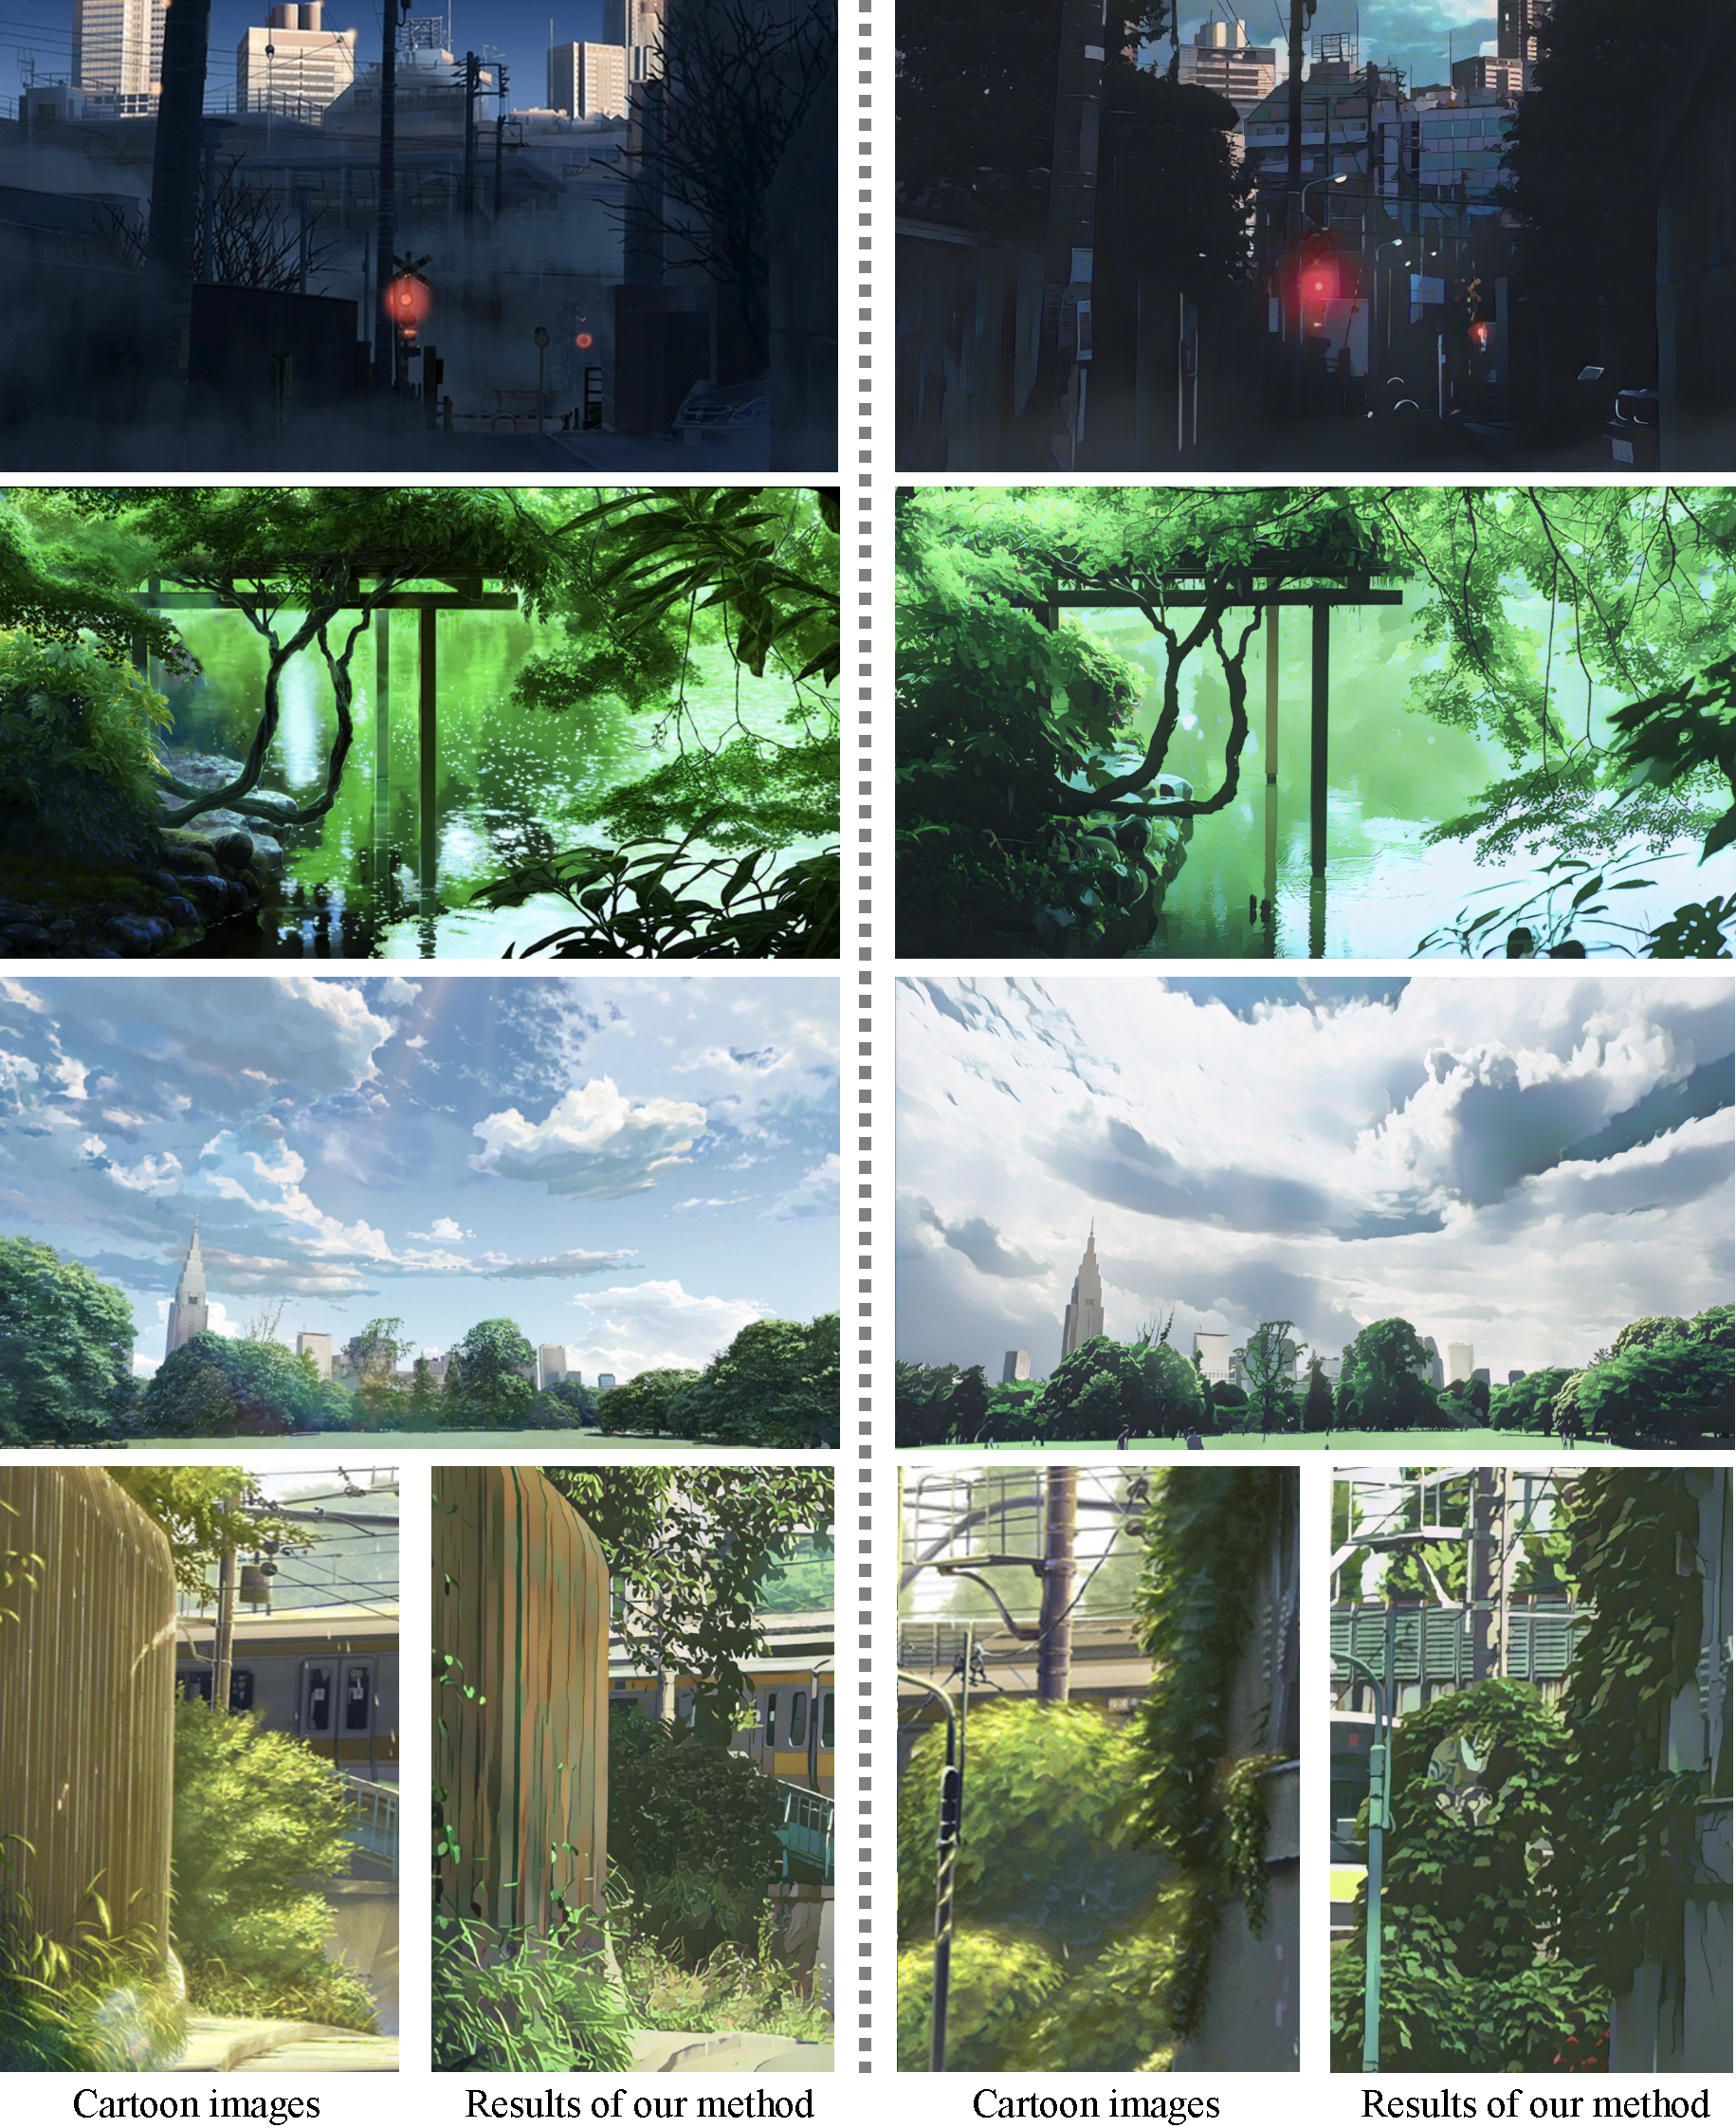
\includegraphics[width=\linewidth]{figures/compare.pdf}
\caption{Comparison between cartoon images and results of our methods in the same scene}
\label{fig:compare1}
\end{figure*}

\begin{figure*}[htb]
\centering
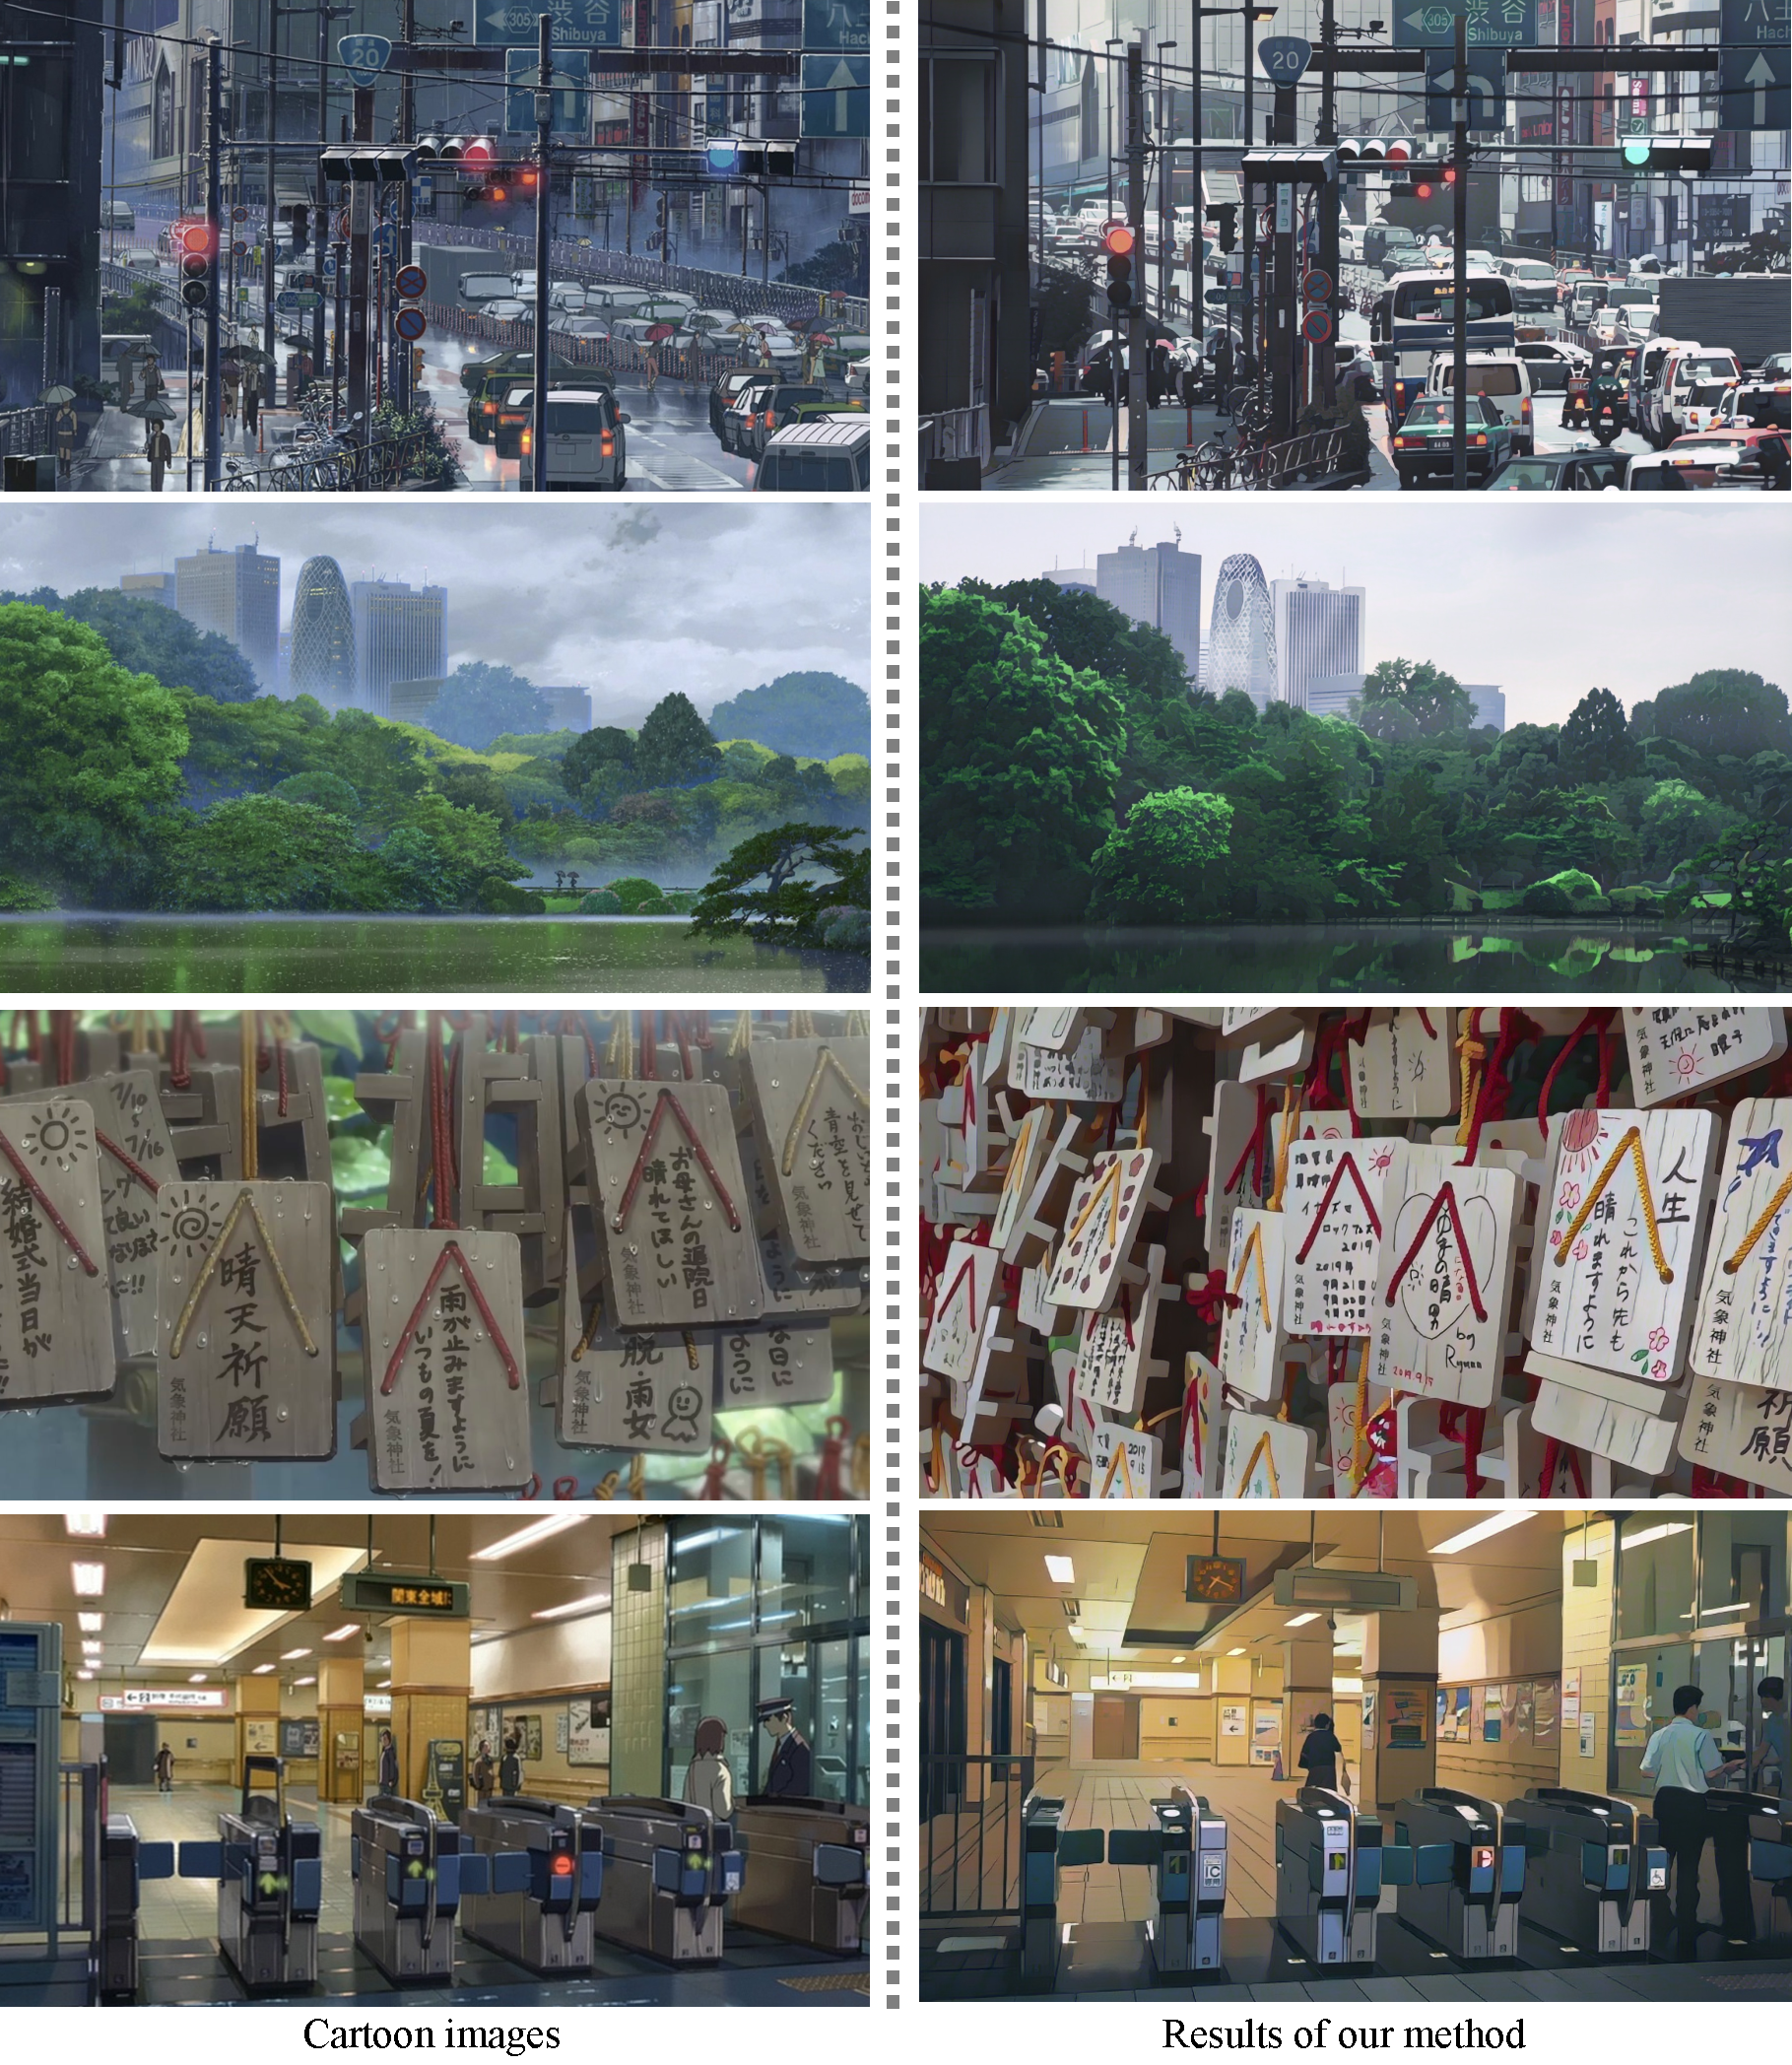
\includegraphics[width=\linewidth]{figures/compare2.pdf}
\caption{Comparison between cartoon images and results of our methods in the same scene.}
\label{fig:compare2}
\end{figure*}
%\clearpage

\begin{figure*}[htb]
\vspace{-0.5em}
\centering
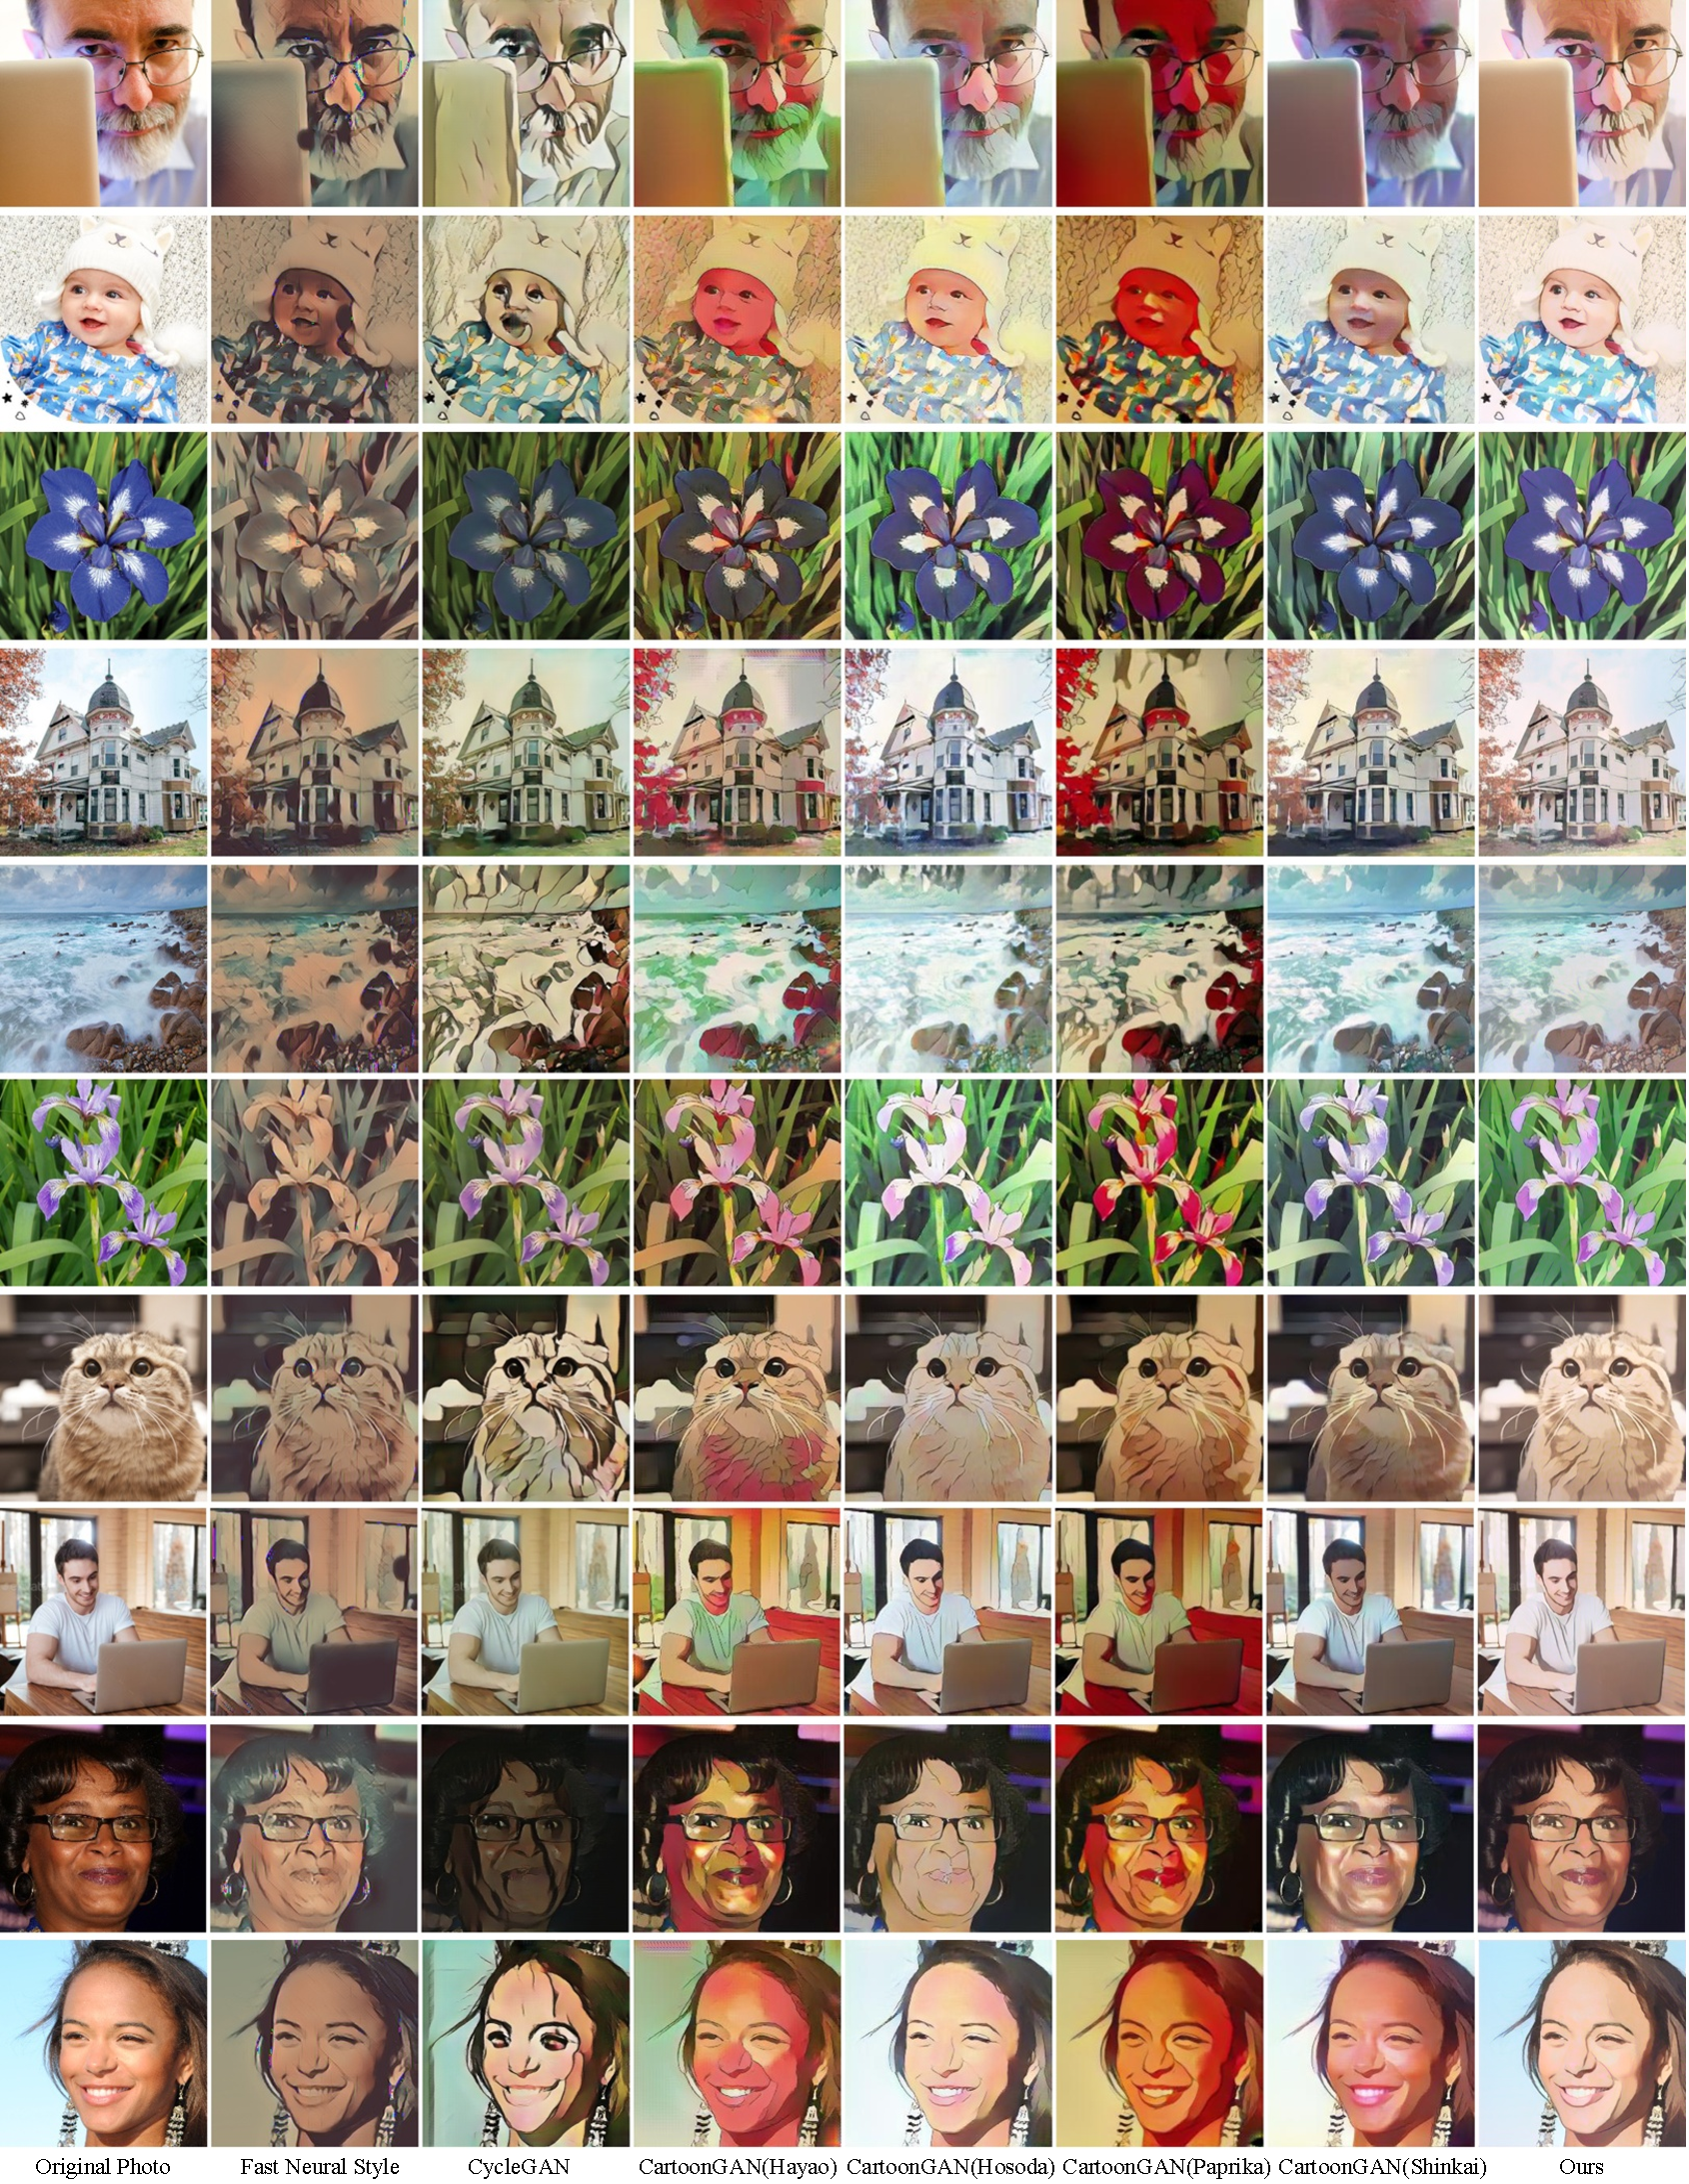
\includegraphics[width=\linewidth]{figures/userstudy1.pdf}
\caption{Some images shown in the user study with scores.}
\label{fig:userstudy1}
\end{figure*}

\begin{figure*}[htb]
%\vspace{-0.5em}
\centering
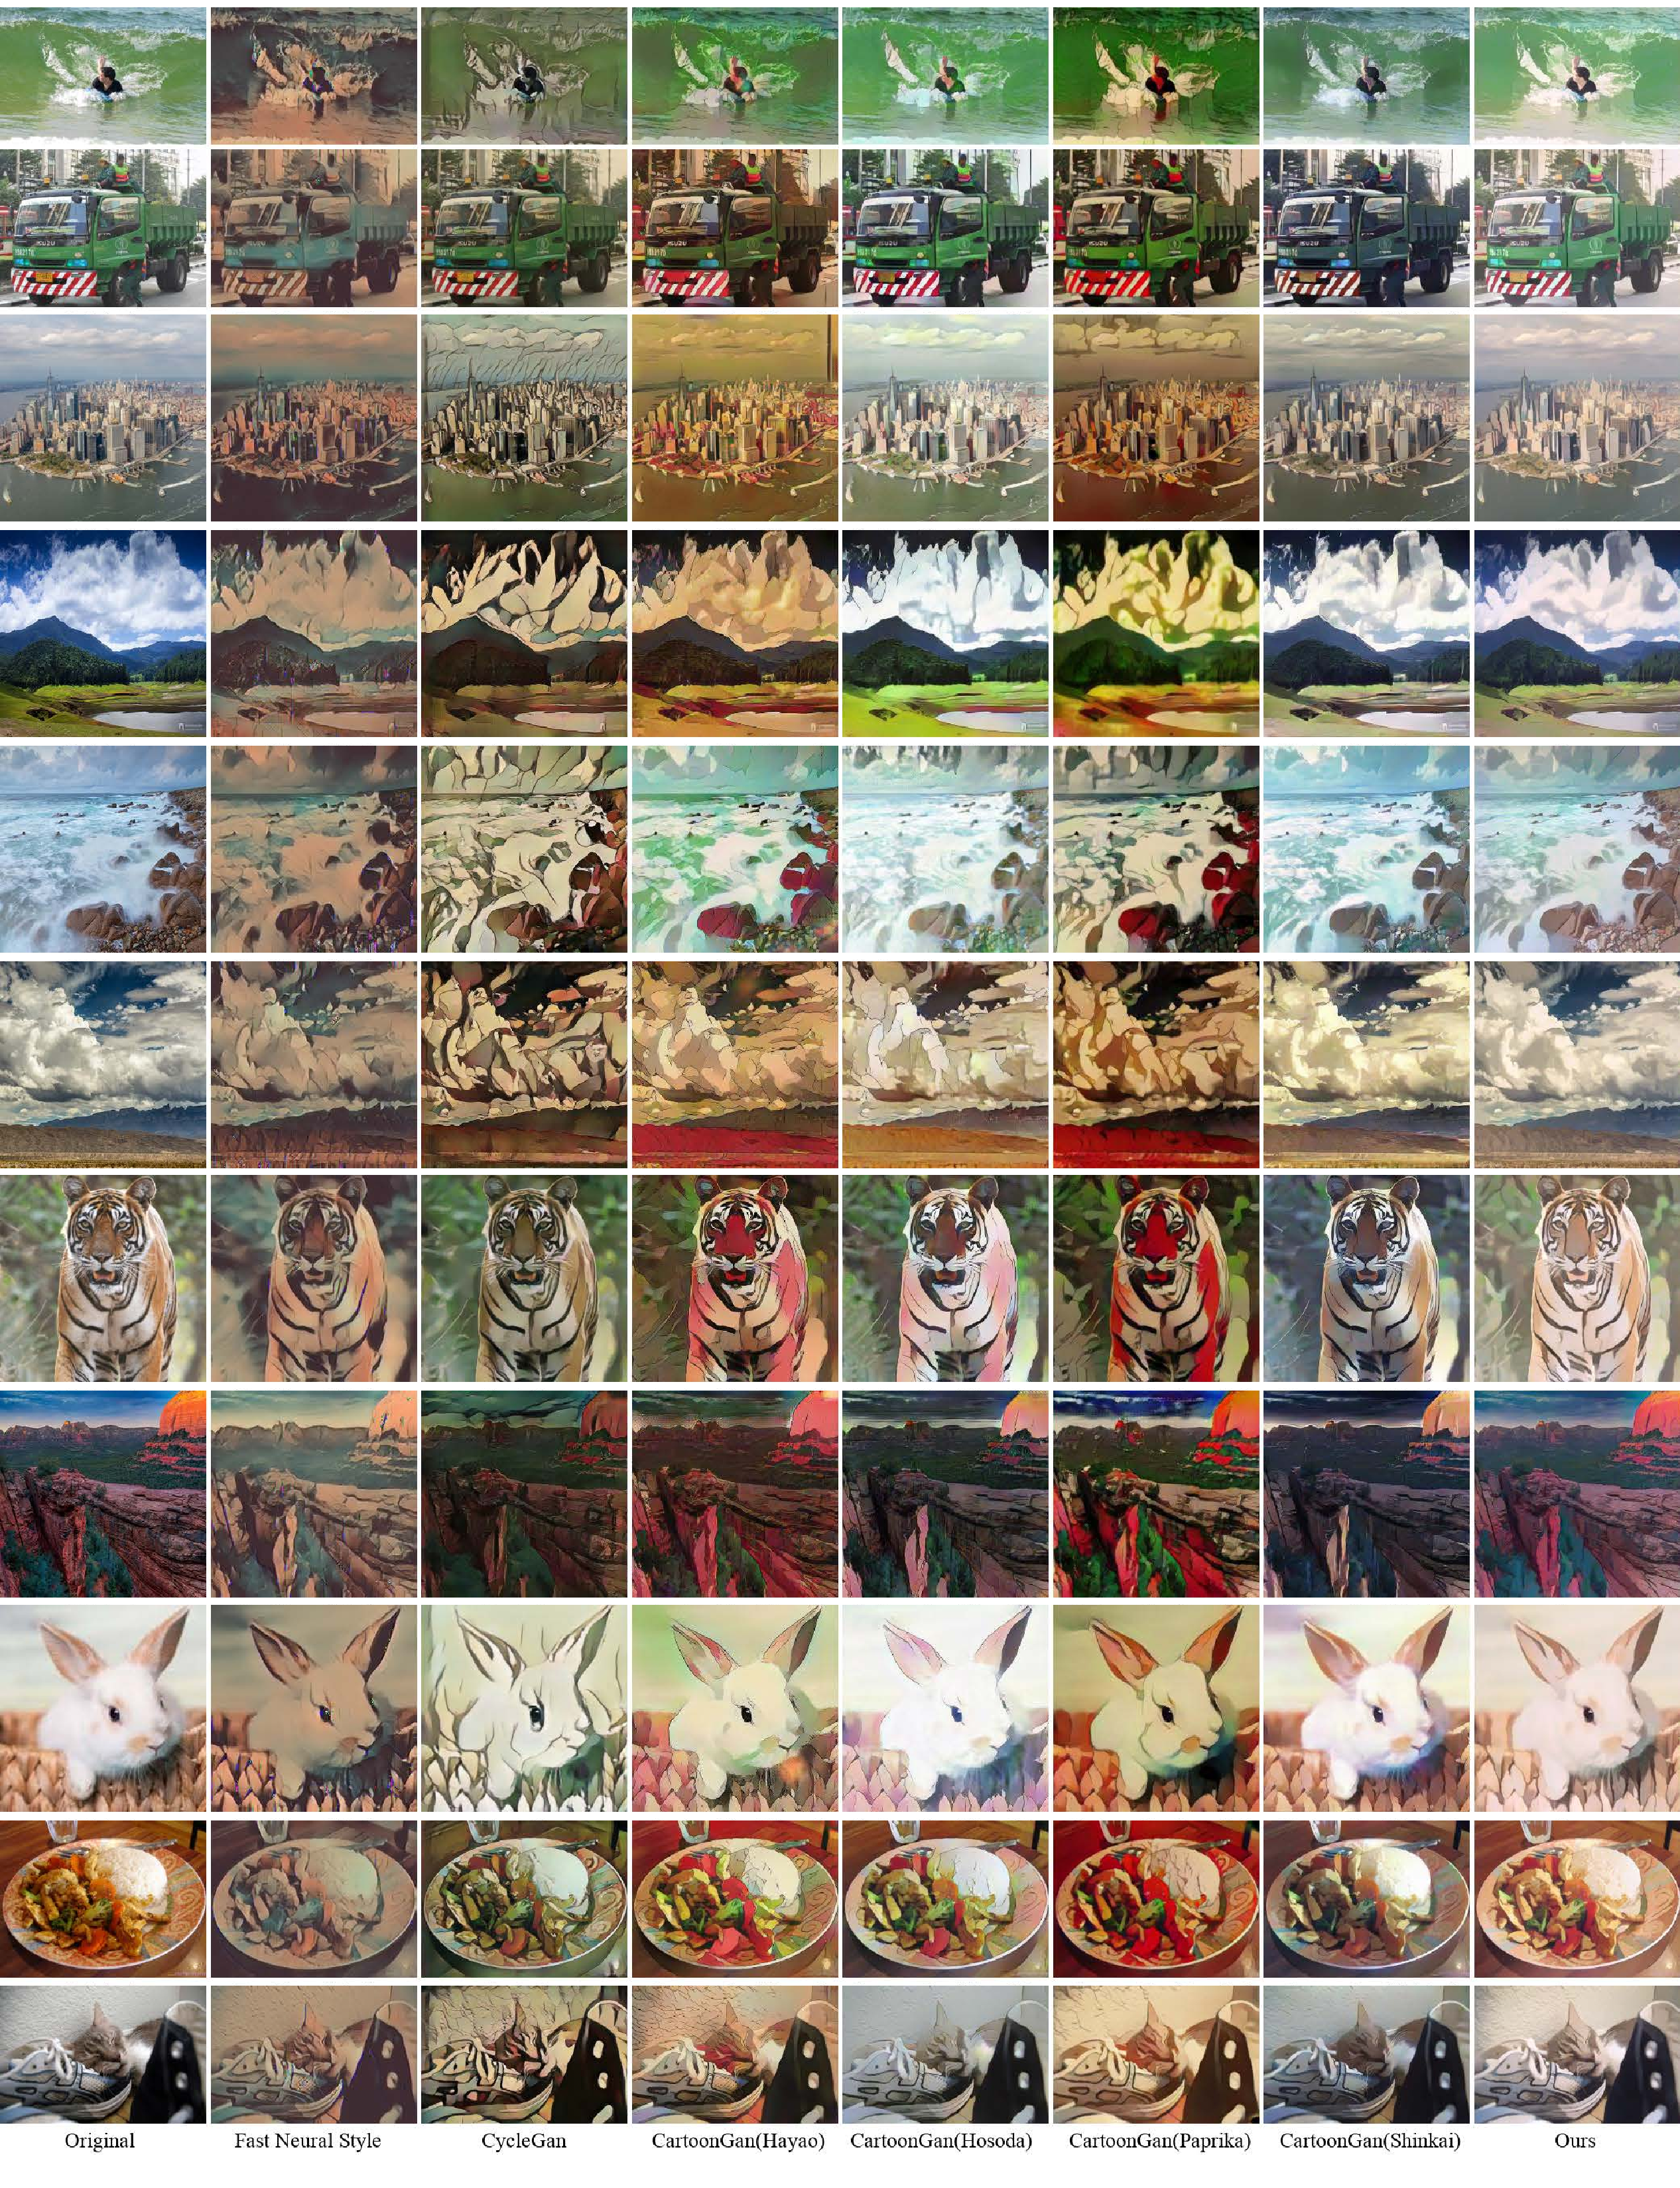
\includegraphics[width=\linewidth]{figures/userstudy2.pdf}
\caption{Images shown in the user study.}
\label{fig:userstudy2}
\end{figure*}

\begin{figure*}[htb]
%\vspace{-0.5em}
\centering
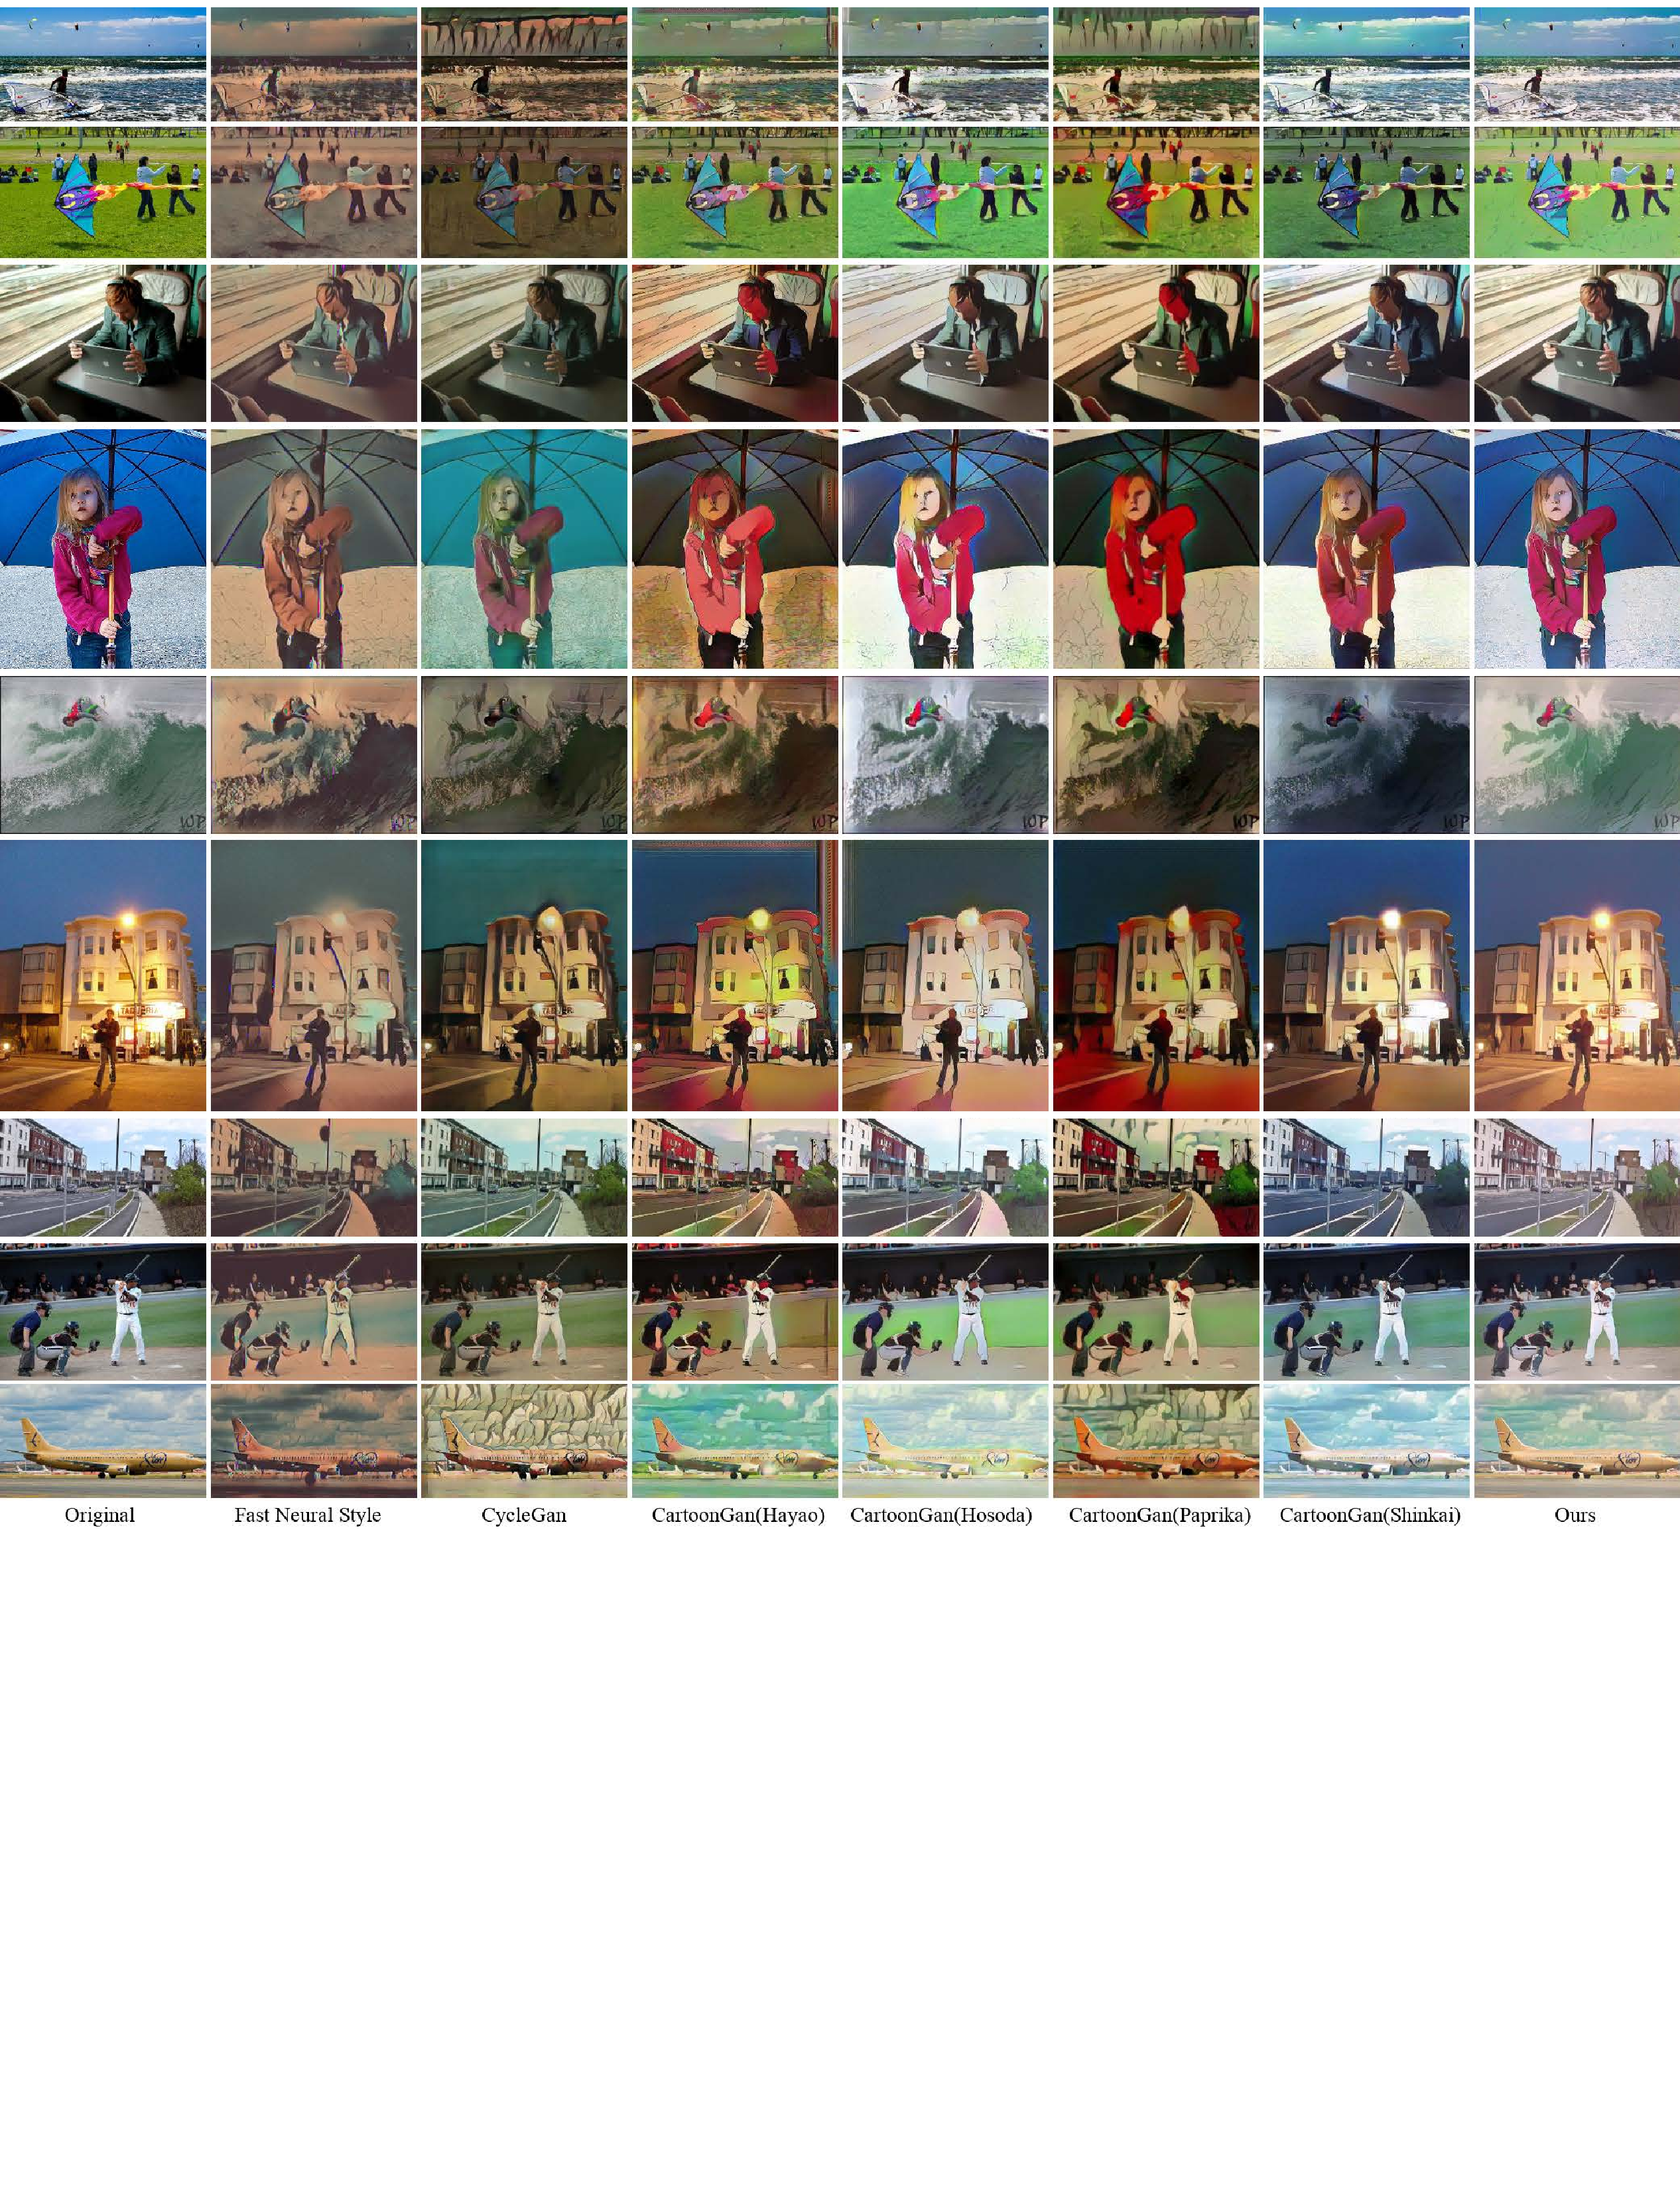
\includegraphics[width=\linewidth]{figures/userstudy3.pdf}
\caption{Images shown in the user study.}
\label{fig:userstudy3}
\end{figure*}

\end{document}
